\documentclass[a4paper,twoside]{article}

\usepackage{epsfig}
\usepackage{subfigure}
\usepackage{calc}
\usepackage{amssymb}
\usepackage{amstext}
\usepackage{amsmath}
\usepackage{amsthm}
\usepackage{multicol}
\usepackage{pslatex}
\usepackage{apalike}
\usepackage{standalone}
\usepackage{longtable}
\usepackage{pbox}
\usepackage[table]{xcolor}
\definecolor{light-gray}{gray}{0.8}
%\rowcolors{1}{magenta}{cyan}
%\rowcolors{1}{}{light-gray}
\let\oldtabular\tabular
\let\endoldtabular\endtabular
\renewenvironment{tabular}{\global\rownum=0\relax\oldtabular}{\endoldtabular}
\usepackage[acronym,toc,nomain]{glossaries}
\makeglossaries
\usepackage{etex}
\usepackage{makecell}
\usepackage{bytefield}
\usepackage{xcolor,colortbl}
\usepackage{a4wide}
\usepackage[inner=1.5in, outer=1.0in, bottom=1in]{geometry}
\usepackage[utf8] {inputenc}
\usepackage[T1] {fontenc}
% \usepackage{amsmath}
\usepackage{amsthm} % is included in mathtools
\newtheorem{theorem}{Theorem}
\usepackage{mathtools}
\usepackage{relsize}
\usepackage{hhline}
\DeclarePairedDelimiter{\ceil}{\lceil}{\rceil}
\DeclarePairedDelimiter{\floor}{\lfloor}{\rfloor}
\usepackage{amsfonts}
\usepackage{verbatim}
\usepackage{todonotes}
\usepackage{calc}
\usepackage{algorithm}
\usepackage{algorithmicx}
\makeatletter
\renewcommand{\ALG@beginalgorithmic}{\scriptsize}
\makeatother
\usepackage{algpseudocode}
\usepackage{multirow}
\usepackage{array}
\usepackage{styles/arydshln}
\usepackage{styles/pgf-umlsd}
\usepackage{pgfgantt}
\algtext*{EndWhile}% Remove "end while" text
\algtext*{EndIf}% Remove "end if" text
\algtext*{EndFor}% Remove "end for" text
\usepackage{caption}
\usepackage{subcaption}
\usepackage{setspace}
\usepackage{pdfpages}
\usepackage{booktabs}
\usepackage{enumitem}
\setitemize{noitemsep}
\usepackage{wrapfig}
\usepackage{pgfplots}
\usepackage{tikz}
\usetikzlibrary{chains}
\usepgflibrary{shapes.geometric}
\usetikzlibrary{shapes}
\usetikzlibrary{calc}
\usetikzlibrary{arrows}
\usetikzlibrary{automata}
\usetikzlibrary{patterns}
\usetikzlibrary{positioning}
\usepackage{styles/tikz-3dplot}
\usepackage{ifthen}
\usepackage{xifthen}
\usepackage{xstring}
\usepackage{pgfopts}
\usepackage{calc}
\usepackage{rotating}
\usepackage{styles/tikz-uml}
\tikzset{
  labelC node/.style={
    at end,align=center,above=-0.08cm,xshift=-6,sloped,
    font=\footnotesize,
    execute at begin node=\setlength{\baselineskip}{0.7em},
    node distance=5cm        
%     append after command={%    
%     \pgfextra
%       \node[draw,near end]{#1};
%       \node[labelB node,middle]{#2}
%       \node[draw,near start]{#3} 
% %      \node[at end, above right]{#2};     
% %      \node[at end, above right]{#3};
%     \endpgfextra
%     }
  },
  labelD node/.style={    
    at start,align=center,sloped,right=-0.08cm,xshift=6,
    rotate=-90,
    font=\footnotesize,
    execute at begin node=\setlength{\baselineskip}{0.7em},
    node distance=5cm        
  }
}
\newcommand{\conceptionalclassbox}[2]{%
\begin{tikzpicture}
\draw (0,0)  node[rectangle,minimum height=0.7cm,draw,minimum width=2.1cm,align=center](satellite){};
\draw (satellite) node[align=center,font=\scriptsize] {#1};
\draw (satellite) node[minimum height=1cm,minimum width=2.1cm,draw,below of=satellite,align=left,font=\scriptsize,node distance =0.85cm](diagram){};
\draw (diagram.north west) node[anchor=north west,align=left,font=\scriptsize] {#2};
\end{tikzpicture}
}
\tikzset{>=stealth',shorten >=1pt,
  object node/.style={
    circle,align=center,
    minimum size=2cm,inner sep=0pt,
    draw
    % font=\sffamily\normalsize\bfseries
  },
  control node/.style={
    circle,dashed,align=center,
    minimum size=2cm,inner sep=0pt,
    draw
    % font=\sffamily\Large\bfseries
  },
  labelA node/.style={
    midway,align=center,above=-0.08cm,sloped,
    font=\footnotesize,
    execute at begin node=\setlength{\baselineskip}{0.7em},
    node distance=5cm
  },
  labelB node/.style={
    midway,align=center,below=-0.08cm,sloped,
    font=\footnotesize,
    execute at begin node=\setlength{\baselineskip}{0.7em},
    node distance=5cm
  },
  labelKrillo node/.style={
    midway,align=center,right=-0.08cm,yshift=2,
    font=\footnotesize,
    execute at begin node=\setlength{\baselineskip}{0.7em},
    node distance=5cm
  },
  labelInvKrillo node/.style={
    midway,align=center,left=-0.08cm,yshift=2,
    font=\footnotesize,
    execute at begin node=\setlength{\baselineskip}{0.7em},
    node distance=5cm
  },
  data node/.style={
    align=center,
    execute at begin node=\setlength{\baselineskip}{1em},
    append after command={%
      \pgfextra
      \draw [-]  (\tikzlastnode.south east) to (\tikzlastnode.south west);
      \draw [-]  (\tikzlastnode.north east) to (\tikzlastnode.north west);
      \endpgfextra
    }
  },
  terminate node/.style={
    align=center,
    execute at begin node=\setlength{\baselineskip}{0.7em}
  },
  task node/.style={
    trapezium,
    trapezium left angle=50,
    trapezium right angle=-50,
    align=center,
    minimum height=1cm, minimum width=4cm, draw,
    append after command={%
    \pgfextra
        \node[draw=none,fill=none, align=center] at (\tikzlastnode.center) {#1};
    \endpgfextra
    }
  },
  harry_potter1 node/.style={
    align=center,minimum height=1.5cm,
    minimum width=0.5cm, rotate=25, anchor = south,
    append after command={%
    \pgfextra
        \node[draw=none,fill=none, align=center] at ([xshift=10, yshift=7]\tikzlastnode.north) (1) {#1};
        \draw  plot [tension=1] coordinates {(\tikzlastnode.north east) ([xshift=5, yshift=-5]\tikzlastnode.center) ([xshift=-5, yshift=5]\tikzlastnode.center) (\tikzlastnode.south west)};
    \endpgfextra
    }
  },
  harry_potter2 node/.style={
    align=center,minimum height=1.5cm,
    minimum width=0.5cm, rotate=25, anchor = south,
    append after command={%
    \pgfextra
        \node[draw=none,fill=none, align=center] at ([xshift=-5, yshift=-10]\tikzlastnode.south) (1) {#1};
        \draw  plot [tension=1] coordinates {(\tikzlastnode.south west) ([xshift=-5, yshift=5]\tikzlastnode.center) ([xshift=5, yshift=-5]\tikzlastnode.center) (\tikzlastnode.north east)};
    \endpgfextra
    }
  },
  queue_v node/.style n args={3}{
    align=center,midway,anchor=center,
    rotate around={#2:(0,0)},
    minimum height = 10, minimum width = 15,
    append after command={%
    \pgfextra
        \draw node[draw=none, fill=white, anchor=south west, rotate=#2, minimum height = 10, minimum width = 15,] at (\tikzlastnode.south west) {};
        \draw node[anchor=north, rotate=90, align=center, font=\footnotesize,
  execute at begin node=\setlength{\baselineskip}{0.9em}] at ([xshift=10]\tikzlastnode.center) {\footnotesize #1};
          \draw[-] plot coordinates {([yshift=#3*4]\tikzlastnode.north west) (\tikzlastnode.south west) (\tikzlastnode.south east) ([yshift=#3*5]\tikzlastnode.north east)};
          \draw[-] plot coordinates {(\tikzlastnode.north east) (\tikzlastnode.north west) (\tikzlastnode.west) (\tikzlastnode.east) (\tikzlastnode.south east)};
    \endpgfextra
    }
  },
  queue_h node/.style n args={3}{
    align=center,midway,anchor=center,
    rotate around={#2:(0,0)},
    minimum height = 15, minimum width = 10,
    append after command={%
    \pgfextra
        \draw node[draw=none, fill=white, anchor=south west, rotate=#2, minimum height = 15, minimum width = 10] at (\tikzlastnode.south west) {};
        \draw node[anchor=south, rotate=0, align=center, font=\footnotesize,execute at begin node=\setlength{\baselineskip}{0.9em}] at ([yshift=8]\tikzlastnode.center) {#1};
          \draw[-] plot coordinates {([xshift=-#3*4]\tikzlastnode.south west) (\tikzlastnode.south east) (\tikzlastnode.north east) ([xshift=-#3*5]\tikzlastnode.north west)};
          \draw[-] plot coordinates {(\tikzlastnode.north west) (\tikzlastnode.south west) (\tikzlastnode.south) (\tikzlastnode.north) (\tikzlastnode.north west)};
    \endpgfextra
    }
  },
  loose_v node/.style n args={3}{
    align=center,midway,anchor=center,
    rotate around={#2:(0,0)},
    minimum height = 10, minimum width = 15,
    append after command={%
    \pgfextra
        \draw node[draw=none, anchor=south west, rotate=#2, minimum height = 10, minimum width = 15,] at (\tikzlastnode.south west) {};
        \draw node[anchor=north, rotate=90, align=center, font=\footnotesize,execute at begin node=\setlength{\baselineskip}{0.9em}] at ([xshift=10]\tikzlastnode.center) {\footnotesize #1};
        \draw[-] plot coordinates {([yshift=#3*4]\tikzlastnode.north west) (\tikzlastnode.south west) (\tikzlastnode.south east) ([yshift=#3*5]\tikzlastnode.north east)};
    \endpgfextra
    }
  },
  loose_h node/.style n args={3}{
    align=center,midway,anchor=center,
    rotate around={#2:(0,0)},
    minimum height = 15, minimum width = 10,
    append after command={%
    \pgfextra
        \draw node[draw=none, anchor=south west, rotate=#2, minimum height = 15, minimum width = 10] at (\tikzlastnode.south west) {};
        \draw node[anchor=south, rotate=0, align=center, font=\footnotesize,execute at begin node=\setlength{\baselineskip}{0.9em}] at ([yshift=8]\tikzlastnode.center) {#1};
          \draw[-] plot coordinates {([xshift=-#3*4]\tikzlastnode.south west) (\tikzlastnode.south east) (\tikzlastnode.north east) ([xshift=-#3*5]\tikzlastnode.north west)};
    \endpgfextra
    }
  },
  reply_h node/.style n args={4}{
    align=center,midway,anchor=center,
    rotate around={#3:(0,0)},
    minimum height = 15, minimum width = 15,
    append after command={%
    \pgfextra
        \draw node[anchor=center, rotate=0, align=center, font=\footnotesize,execute at begin node=\setlength{\baselineskip}{0.9em}] at ([yshift=(#4*16)+#4*16]\tikzlastnode.center) {\footnotesize #1};
        \draw node[anchor=center, rotate=0, align=center, font=\footnotesize,execute at begin node=\setlength{\baselineskip}{0.9em}] at ([yshift=-#4*22]\tikzlastnode.center) {\footnotesize #2};
        \draw[-] plot coordinates {(\tikzlastnode.south east) (\tikzlastnode.south west) (\tikzlastnode.north west) (\tikzlastnode.north east) ([yshift=#4*15]\tikzlastnode.north east) ([yshift=#4*15,xshift=-#4*16]\tikzlastnode.north east)};
    \endpgfextra
    }
  },
  reply_v node/.style n args={4}{
    align=center,midway,anchor=center,
    rotate around={#3:(0,0)},
    minimum height = 15, minimum width = 15,
    append after command={%
    \pgfextra
        \draw node[anchor=west, rotate=0, align=center, font=\footnotesize,execute at begin node=\setlength{\baselineskip}{0.9em}] at ([xshift=(1+#4)*-24+(1-#4)*8]\tikzlastnode.west) {\footnotesize #1};
        \draw node[anchor=east, rotate=0, align=center, font=\footnotesize, execute at begin node=\setlength{\baselineskip}{0.9em}] at ([xshift=(1+#4)*15]\tikzlastnode.east) {\footnotesize #2};
        \draw[-] plot coordinates {(\tikzlastnode.north east) (\tikzlastnode.south east) (\tikzlastnode.south west) (\tikzlastnode.north west) ([xshift=-#4*15]\tikzlastnode.north west) ([xshift=-#4*15,yshift=-#4*16]\tikzlastnode.north west)};
    \endpgfextra
    }
  },
  data node/.style={
    rectangle,align=center,
    minimum width=2cm,minimum height=1.cm,
    inner sep=0pt,
    draw
   },
   start node/.style={
     circle,fill=black,align=center,
     minimum size=0.75cm,inner sep=0pt,draw
  },
  end node/.style={
     circle, align=center, minimum size=0.75cm, draw,
     append after command = {
     \pgfextra
        \draw node[circle, align=center, minimum size = 0.5cm, fill=black] at (\tikzlastnode.center) {};
     \endpgfextra
     }
  },
  single_queue_v node/.style n args={3}{
    align=center,midway,anchor=center,
    rotate around={#2:(0,0)},
    minimum height = 10, minimum width = 15,
    append after command={%
    \pgfextra
        \draw node[draw=none, fill=white, anchor=south west, rotate=#2, minimum height = 4, minimum width = 15,] at (\tikzlastnode.south west) {};
        \draw node[anchor=north, rotate=90, align=center, font=\footnotesize,
  execute at begin node=\setlength{\baselineskip}{0.9em}] at ([xshift=10]\tikzlastnode.center) {\footnotesize #1};
          \draw[-] plot coordinates {([yshift=#3*4]\tikzlastnode.north west) (\tikzlastnode.south west) (\tikzlastnode.south east) ([yshift=#3*5]\tikzlastnode.north east)};
          \draw[-] plot coordinates { ([yshift=-4]\tikzlastnode.north west) ([yshift=-4]\tikzlastnode.north east) ([yshift=0]\tikzlastnode.south east)};
    \endpgfextra
    }
  }
}

\usepackage{ellipsis}
\usetikzlibrary{calc}
\usetikzlibrary{decorations.pathreplacing,decorations.markings,shapes.geometric}
\tikzset{naming/.style={align=center,font=\small}}
\tikzset{antenna/.style={insert path={-- coordinate (ant#1) ++(0,0.25) -- +(135:0.25) + (0,0) -- +(45:0.25)}}}
\tikzset{station/.style={naming,draw,shape=dart,shape border rotate=90, minimum width=10mm, minimum height=10mm,outer sep=0pt,inner sep=3pt}}
%\tikzset{mobile/.style={naming,draw,shape=rectangle,minimum width=15mm,minimum height=7.5mm, outer sep=0pt,inner sep=3pt}}
\tikzset{mobile/.style={naming,draw,shape=rectangle,minimum width=12mm,minimum height=6mm, outer sep=0pt,inner sep=3pt}}
\tikzset{radiation/.style={{decorate,decoration={expanding waves,angle=90,segment length=4pt}}}}

\newcommand{\MUE}[1]{%
\begin{tikzpicture}[every node/.append style={rectangle,minimum width=0pt}]
\node [mobile,label={[inner ysep=+.3333em]\dots}] (box) {#1};

%\node [mobile] (box) {#1};
%\node at ($(ant1)!0.5!(ant2)$) {\dots};

\draw ([xshift=.25cm] box.south west) circle (4pt)
      ([xshift=-.25cm]box.south east) circle (4pt);

\fill ([xshift=.25cm] box.south west) circle (1pt)
      ([xshift=-.25cm]box.south east) circle (1pt);

\draw ([xshift=.25cm] box.north west) [antenna=1];
\draw ([xshift=-.25cm]box.north east) [antenna=2];
\end{tikzpicture}
}

\newcommand{\UE}[1]{%
\begin{tikzpicture}[every node/.append style={rectangle,minimum width=0pt}]
\node[mobile] (box) {#1};

\draw ([xshift=.25cm] box.south west) circle (4pt)
      ([xshift=-.25cm]box.south east) circle (4pt);

\fill ([xshift=.25cm] box.south west) circle (1pt)
      ([xshift=-.25cm]box.south east) circle (1pt);

\draw (box.north) [antenna=1];
\end{tikzpicture}
}

\newcommand{\MBS}[1]{%
\begin{tikzpicture}
\node[station] (base) {#1};

%\draw[line join=bevel] (base.110) -- (base.70) -- (base.north west) -- (base.north east) -- cycle;
\draw[line join=bevel] (base.100) -- (base.80) -- (base.110) -- (base.70) -- (base.north west) -- (base.north east);
\draw[line join=bevel] (base.100) -- (base.70) (base.110) -- (base.north east);

% original yshift=.8pt
%\draw[line cap=rect] ([xshift=.5cm,yshift=.3pt] base.north) [antenna=1];
%\draw[line cap=rect] ([yshift=.3pt]ant1 |- base.north) -- node[above,shape=rectangle,inner ysep=+.3333em]{\dots} ([xshift=-.5cm,yshift=.3pt]base.north) [antenna=2];
\draw[line cap=rect] ([xshift=-.1768cm,yshift=.6pt]base.north -| base.right tail) [antenna=1];
\draw[line cap=rect] ([yshift=.6pt]ant1 |- base.north) -- node[above,shape=rectangle,inner ysep=+.3333em]{\dots} ([xshift=.1768cm,yshift=.6pt]base.north -| base.left tail) [antenna=2];

%\draw[line cap=rect] ([yshift=.3pt]ant1 |- base.north) -- ([xshift=-.5cm,yshift=.3pt]base.north) [antenna=2];
%\node at ($(ant1)!0.5!(ant2)$) {\dots};
\end{tikzpicture}
}

\newcommand{\BS}[1]{%
\begin{tikzpicture}
\node[station] (base) {#1};

%\draw[line join=bevel] (base.110) -- (base.70) -- (base.north west) -- (base.north east) -- cycle;
\draw[line join=bevel] (base.100) -- (base.80) -- (base.110) -- (base.70) -- (base.north west) -- (base.north east);
\draw[line join=bevel] (base.100) -- (base.70) (base.110) -- (base.north east);

% original yshift=.8pt
\draw[line cap=rect] ([yshift=0pt]base.north) [antenna=1];
\end{tikzpicture}
}

\newcommand{\BSSIMPLE}[1]{%
\begin{tikzpicture}
\node[station] (base) {#1};

%\draw[line join=bevel] (base.110) -- (base.70) -- (base.north west) -- (base.north east) -- cycle;
\draw[line join=bevel] (base.100) -- (base.80) -- (base.110) -- (base.70) -- (base.north west) -- (base.north east);
\draw[line join=bevel] (base.100) -- (base.70) (base.110) -- (base.north east);

\end{tikzpicture}
}
\tikzset{>=stealth',shorten >=1pt,
  computer node/.style={
        rectangle, align=center,
        minimum width=1.4cm,minimum height=1.3cm,draw,
        append after command={
        \pgfextra
        \draw node[draw,minimum width=1.2cm,minimum height=1.1cm] at (\tikzlastnode.center) {};
        \draw node[draw,minimum width=1.5cm,minimum height=0.6cm] at ([yshift=-0.4cm]\tikzlastnode.south) {};
        \draw node[circle, fill=black, minimum size=0.15cm, inner sep=0pt] at ([xshift=0.55cm,yshift=-0.25cm]\tikzlastnode.south) {};
        \endpgfextra
      }
  }
}
\newsavebox{\documentt}
\savebox{\documentt}{
  \begin{tikzpicture}
    \draw (3,4) -- (3,2.75) to[out=-100,in=100] (5,2.75) -- (5,4) -- (3,4);
    % \draw (0,0) -- (1,-0.1666666);
    % \draw (-1.2,0.2) -- (-2.2,0.366666);
    % \draw (-1,0) -- (-2,-0.1666666);
    % \draw (-0.2,0.2) -- (0.8,0.366666);
  \end{tikzpicture}
}


\newsavebox{\cubesatbox}
\savebox{\cubesatbox}{
  \begin{tikzpicture}
    \draw (0,0) rectangle(-1,-1)
    -- (-1.2,-0.8) -- (-1.2,0.2) -- (-1,0) -- (-1.2,0.2)
    -- (-0.2,0.2) -- (0,0);
    \draw (0,0) -- (1,-0.1666666);
    \draw (-1.2,0.2) -- (-2.2,0.366666);
    \draw (-1,0) -- (-2,-0.1666666);
    \draw (-0.2,0.2) -- (0.8,0.366666);
  \end{tikzpicture}
}

\newcommand{\documentTikz}[1]{\scalebox{#1}{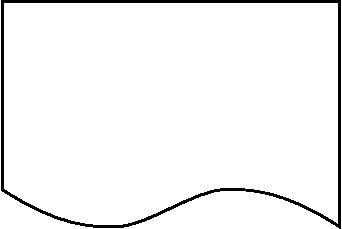
\includegraphics{styles/document.pdf}}}

\usepackage{epstopdf}

\tikzset{
  ciscorouter/.style={align=center,label={center:
      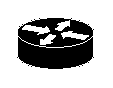
\includegraphics[]{styles/cisco/router.eps}
    },minimum width=0.9cm,minimum height=0.9cm}
}
\tikzset{
  ciscotap/.style={align=center,label={center:
      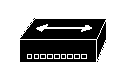
\includegraphics[]{styles/cisco/smallhub.eps}
    },minimum width=0.9cm,minimum height=0.9cm}
}

\usepackage{circuitikz}
\usepackage{multicol}
\newcommand*{\tabbox}[2][t]{\vspace{0pt}\parbox[#1][3.7\baselineskip]{1cm}{\strut#2\strut}}
\usepackage{float}
\usepackage{graphicx}
\usepackage{tabu}
\usepackage{lastpage}
\usepackage{lmodern}
\usepackage[toc,page]{appendix}
\usepackage[titles]{tocloft}
\usepackage{listings}
\usepackage{DejaVuSansMono}
\usepackage{tabularx}
\usepackage{fancyhdr}
\usepackage{cancel}
\setlength{\headheight}{15pt}
\pagestyle{fancyplain}
\usepackage{chngcntr}
\usepackage{footnote}
\makesavenoteenv{tabular}
\makesavenoteenv{table}
\counterwithout{footnote}{chapter}
\usepackage[hang,flushmargin,multiple]{footmisc}
\fancyhf{} % Ingen linje
% Skriv kapitelnavn som lowercase
\renewcommand{\chaptermark}[1]{\markboth{#1}{}}
\lhead[\fancyplain{}{\textit{\thechapter.\ \leftmark}}]{}
\rhead[]{\fancyplain{}{\textit{\leftmark\ \thechapter.}}}
\rfoot[]{\thepage}
\lfoot[\thepage]{}

\definecolor{lightgray}{gray}{0.90}
\newcommand{\colorbitbox}[3]{%
\rlap{\bitbox{#2}{\color{#1}\rule{\width}{\height}}}%
\bitbox{#2}{#3}}

\setcounter{tocdepth}{1}

%\renewcommand{\appendixname}{Bilag}
%\renewcommand{\appendixpagename}{Bilag}
%\renewcommand{\appendixtocname}{Bilag}

\usepackage{caption}
\captionsetup{font=footnotesize,labelfont=bf}
\captionsetup[figure]{labelfont=bf}
\usepackage{titlesec}
\titleformat{\chapter}{\normalfont\LARGE\bfseries}{\thechapter}{1em}{}
\titlespacing*{\chapter}{0pt}{-50pt}{20pt}
%\captionsetup[lstlisting]{labelfont=bf}
\usepackage{MnSymbol}
%\lstset{basicstyle=\scriptsize, tabsize=2, captionpos=b, frame=single}
\lstset{prebreak=\raisebox{0ex}[0ex][0ex]{\ensuremath{\rhookswarrow}}}
\lstset{breaklines=true, breakatwhitespace=true}
\renewcommand{\lstlistingname}{Code}

\lstset{
  language=c,
  basicstyle=\ttfamily\scriptsize,
  identifierstyle=\ttfamily,
  keywordstyle=\ttfamily,
  numbers=left,
  numbersep=5pt,
  xleftmargin=20pt,
  frame=tb,
  framexleftmargin=20pt,
  showstringspaces=false
}

\renewcommand*\thelstnumber{\arabic{lstnumber}:}

\DeclareCaptionFormat{mylst}{\hrule#1#2#3}
\captionsetup[lstlisting]{format=mylst,labelfont=bf,singlelinecheck=off,labelsep=space}


\usepackage{suffix}
\newcommand{\algoref}[1]{Algorithm~\ref{alg:#1}}
\newcommand{\appendixref}[1]{Appendix~-~\emph{\nameref{app:#1}}}
\newcommand{\appendixfigref}[2]{Appendix~\emph{\nameref{app:#1}~-~Figure~\ref{fig:#2}}}
\WithSuffix\newcommand\appendixref*[1]{Appendix~-~\emph{\nameref{app:#1}}}
%\newcommand{\@@appendixref}[1]{Appendix~\emph{\ref{app:#1}}}
\newcommand{\reqref}[1]{Req. \ref{req:#1_long}}
\newcommand{\reqrefnotext}[1]{Req. \ref{req:#1}}
\newcommand{\reqrefshort}[1]{\ref{req:#1_long}}
\newcommand{\reqrefshortnotext}[1]{\ref{req:#1}}
\captionsetup[subfigure]{labelformat=parens}
\newcommand{\subfigref}[1]{(\subref{fig:#1})}
\newcommand{\sectionref}[1]{Section~\emph{\ref{sec:#1}~\nameref{sec:#1}}}
\WithSuffix\newcommand\sectionref*[1]{Section~\emph{\ref{sec:#1}}}
\newcommand{\chapterref}[1]{Chapter~\emph{\ref{sec:#1}~\nameref{sec:#1}}}
\WithSuffix\newcommand\chapterref*[1]{Chapter~\emph{\ref{sec:#1}}}
\newcommand{\figref}[1]{Figure~\ref{fig:#1}}
\newcommand{\listingref}[1]{\lstlistingname~\ref{lst:#1}}
\newcommand{\tableref}[1]{Table~\ref{tab:#1}}
\newcommand{\theoremref}[1]{Theorem~\ref{th:#1}}
\newcommand{\equationref}[1]{Equation~\ref{eq:#1}}


\newcounter{req_counter}
\setcounter{req_counter}{1}

\makeatletter
\newcommand{\reqlabel}[2]{%
  \label{#1}
  \protected@write \@auxout {}{\string \newlabel {#1_long}{{\ref{#1} (#2)}{\thepage}{#2}{#1}{}}}%
  \hypertarget{#1}{#2}
}
\makeatother

\newcommand{\fullfigure}[3]{
  \begin{figure}[ht]
    \centering
    \includegraphics[width=.95\textwidth]{#1}
    \caption{#3}
    \label{fig:#2}
  \end{figure}
}

\newcommand{\fullfigurehere}[3]{
  \begin{figure}[H]
    \centering
    \includegraphics[width=.95\textwidth]{#1}
    \caption{#3}
    \label{fig:#2}
  \end{figure}
}

\newcommand{\fullfigureimport}[3]{
  \begin{figure}[ht]
    \centering
    \input{#1}
    \ifthenelse{\equal{#3}{}}{}{
      \caption{#3}
    }
    \ifthenelse{\equal{#2}{}}{}{
      \label{fig:#2}
    }
  \end{figure}
}

\newcommand{\largefigureimport}[3]{
  \begin{figure}[ht]
    \centering
    \scalebox{0.8}{\input{#1}}
    \ifthenelse{\equal{#3}{}}{}{
      \caption{#3}
    }
    \ifthenelse{\equal{#2}{}}{}{
      \label{fig:#2}
    }
  \end{figure}
}

\newcommand{\mediumfigureimport}[3]{
  \begin{figure}[ht]
    \centering
    \scalebox{0.66}{\input{#1}}
    \ifthenelse{\equal{#3}{}}{}{
      \caption{#3}
    }
    \ifthenelse{\equal{#2}{}}{}{
      \label{fig:#2}
    }
  \end{figure}
}

\newcommand{\smallfigureimport}[3]{
  \begin{figure}[ht]
    \centering
    \scalebox{0.50}{\input{#1}}
    \ifthenelse{\equal{#3}{}}{}{
      \caption{#3}
    }
    \ifthenelse{\equal{#2}{}}{}{
      \label{fig:#2}
    }
  \end{figure}
}

\newcommand{\tinyfigureimport}[3]{
  \begin{figure}[ht]
    \centering
    \scalebox{0.25}{\input{#1}}
    \ifthenelse{\equal{#3}{}}{}{
      \caption{#3}
    }
    \ifthenelse{\equal{#2}{}}{}{
      \label{fig:#2}
    }
  \end{figure}
}

\newcommand{\fullfigureimporthere}[3]{
  \begin{figure}[H]
    \centering
    \input{#1}
    \ifthenelse{\equal{#3}{}}{}{
      \caption{#3}
    }
    \ifthenelse{\equal{#2}{}}{}{
      \label{fig:#2}
    }
  \end{figure}
}

\newcommand{\fullfigureimporttop}[3]{
  \begin{figure}[t]
    \centering
    \input{#1}
    \ifthenelse{\equal{#3}{}}{}{
      \caption{#3}
    }
    \ifthenelse{\equal{#2}{}}{}{
      \label{fig:#2}
    }
  \end{figure}
}

\newcommand{\fullpagefigure}[3]{
  \begin{figure}[hbtp]
    \centering
    \includegraphics{#1}
    \caption{#3}
    \label{fig:#2}
  \end{figure}
}


\newcommand{\fullpagefigureimport}[3]{
  \begin{figure}[hbtp]
    \centering
    \input{#1}
    \caption{#3}
    \label{fig:#2}
  \end{figure}
}

\newcommand{\smallfigure}[3]{
  \begin{figure}[ht]
    \centering
    \includegraphics[width=.55\textwidth,height=.55\textwidth,keepaspectratio]{#1}
    \caption{#3}
    \label{fig:#2}
  \end{figure}
}

\newcommand{\smallerfigure}[3]{
  \begin{figure}[ht]
    \centering
    \includegraphics[width=.50\textwidth,height=.55\textwidth,keepaspectratio]{#1}
    \caption{#3}
    \label{fig:#2}
  \end{figure}
}

\newcommand{\tinyfigure}[3]{
  \begin{figure}[ht]
    \centering
    \includegraphics[width=.25\textwidth,height=.25\textwidth,keepaspectratio]{#1}
    \caption{#3}
    \label{fig:#2}
  \end{figure}
}


\newcommand{\mediumfigure}[3]{
  \begin{figure}[ht]
    \centering
    \includegraphics[width=.65\textwidth,height=.65\textwidth,keepaspectratio]{#1}
    \caption{#3}
    \label{fig:#2}
  \end{figure}
}

\newcommand{\largefigure}[3]{
  \begin{figure}[ht]
    \centering
    \includegraphics[width=.75\textwidth,height=.75\textwidth,keepaspectratio]{#1}
    \caption{#3}
    \label{fig:#2}
  \end{figure}
}

\newcommand{\largerfigure}[3]{
  \begin{figure}[ht]
    \centering
    \includegraphics[width=.85\textwidth,height=.85\textwidth,keepaspectratio]{#1}
    \caption{#3}
    \label{fig:#2}
  \end{figure}
}

\newcommand{\evenlargerfigure}[3]{
  \begin{figure}[ht]
    \centering
    \includegraphics[width=.99\textwidth,height=.95\textwidth,keepaspectratio]{#1}
    \caption{#3}
    \label{fig:#2}
  \end{figure}
}

\newcommand{\largestfigure}[3]{
  \begin{figure}[ht]
    \centering
    \includegraphics[width=1.05\textwidth,height=1.05\textwidth,keepaspectratio]{#1}
    \caption{#3}
    \label{fig:#2}
  \end{figure}
}


% \twofigures{width}{fig1name}{fig1label}{fig1caption}{fig2name}{fig2label}{fig2caption}{overall_label}{overall_caption}
\newcommand{\twofigures}[9]{
  \begin{figure}[H]
	\centering
	\begin{subfigure}[b]{#1\textwidth}
		\centering
		\includegraphics[width=\textwidth]{#2}
		\caption{#4}
        \label{fig:#3}
	\end{subfigure}
    \quad
	\begin{subfigure}[b]{#1\textwidth}
		\centering
		\includegraphics[width=\textwidth]{#5}
		\caption{#7}
        \label{fig:#6}
	\end{subfigure}
	\caption{#9}
    \label{fig:#8}
  \end{figure}
}

% \threefigures{width}{fig1name}{fig1caption}{fig2name}{fig2caption}{fig3name}{fig3caption}{fig4name}{fig4caption}{fig5name}{fig5caption}{overall_label}{overall_caption}
\newcommand{\threefigures}[9]{
  \begin{figure}[H]
	\centering
	\begin{subfigure}[b]{#1\textwidth}
		\centering
		\includegraphics[width=\textwidth]{#2}
		\caption{#3}
        \label{fig:#2}
	\end{subfigure}
    \quad
	\begin{subfigure}[b]{#1\textwidth}
		\centering
		\includegraphics[width=\textwidth]{#4}
		\caption{#5}
        \label{fig:#4}
	\end{subfigure}
    \quad
	\begin{subfigure}[b]{#1\textwidth}
		\centering
		\includegraphics[width=\textwidth]{#6}
		\caption{#7}
        \label{fig:#6}
	\end{subfigure}
	\caption{#9}
    \label{fig:#8}
  \end{figure}
}



% Bibliography
\bibliographystyle{IEEE}

\usepackage[footnote,draft,danish,silent,nomargin]{fixme}
\newcommand{\unit}[1]{~\text{#1}}
\newcommand{\rom}[1]{\uppercase\expandafter{\romannumeral #1}}

\newacronym{cnn}{CNN}{Convolutional Neural Network}
\newacronym{pascalvoc}{PASCAL VOC}{Pattern Analysis, Statistical Modelling and Computational Learning Visual Object Classes}
\newacronym{mscoco}{MS COCO}{Microsoft Common Objects in Context}
\newacronym{ilsvrc}{ILSVRC}{ImageNet Large Scale Visual Recognition Challenge}
\newacronym{svm}{SVM}{Support Vector Machine}
\newacronym{nms}{NMS}{Non-maximum Suppression}
\newacronym{map}{mAP}{Mean Average Precision}
\newacronym{roi}{RoI}{Region of Interest}
\newacronym{rpn}{RPN}{Region Proposal Network}
\newacronym{iou}{IoU}{Intersection-Over-Union}
\newacronym{ssd}{SSD}{Single Shot Detector}
\newacronym{yolo}{YOLO}{You Only Look Once}
\newacronym{fcn}{FCN}{Fully Convolutional Network}
\newacronym{rfcn}{R-FCN}{Region-based Fully Convolutional Network}
\newacronym{ion}{ION}{Inside-Outside Net}
\newacronym{rnn}{RNN}{Recurrent Neural Network}
\newacronym{tdm}{TDM}{Top-down Modulation}
\newacronym{fcis}{FCIS}{Fully Convolutional Instance-aware Segmentation}
\newacronym{ohem}{OHEM}{Online Hard Example Mining}
\newacronym{sgd}{SGD}{Stochastic Gradient Descent}
\newacronym{relu}{ReLU}{Rectified Linear Unit}
\newacronym{flops}{FLOPs}{Floating Point Operations}
\newacronym{ap}{AP}{Average Precision}
\newacronym{caffe}{Caffe}{Convolutional Architecture for Fast Feature Embedding}
\newacronym{iqa}{IQA}{Image Quality Assessment}
\newacronym{nr}{NR}{No-Reference}
\newacronym{live}{LIVE}{Laboratory for Image \& Video Engineering}
\newacronym{lcc}{LCC}{Pearson Linear Correlation Coefficient}
\newacronym{srocc}{SROCC}{Spearman Rank Order Coefficient}
\newacronym{ff}{FF}{Fast Fading}
\newacronym{bpp}{BPP}{Bits per Pixel}
\newacronym{dmos}{DMOS}{Difference Mean Opinion Score}
\newacronym{ar}{AR}{Average Recall}
\newacronym{friqa}{FR-IQA}{Full-Reference Image Quality Assessment}
\newacronym{nriqa}{NR-IQA}{No-Reference Image Quality Assessment}
\usepackage{SCITEPRESS}     % Please add other packages that you may need BEFORE the SCITEPRESS.sty package.



\subfigtopskip=0pt
\subfigcapskip=0pt
\subfigbottomskip=0pt

\begin{document}

\title{R-FCN Object Detection Ensemble based on Object Resolution and Image Quality}

\author{\authorname{Christoffer B{\o}gelund Rasmussen\sup{1} and Kamal Nasrollahi\sup{1}}
\affiliation{\sup{1}Visual Analysis of People (VAP) Laboratory, Aalborg University, Aalborg, Denmark}
\email{cbra12@student.aau.dk, kn@create.aau.dk}
}

\keywords{Convolutional Neural Networks, Object Detection, Image Quality Assessment, Ensemble Learning.}

\abstract{Object detection can be difficult due to challenges such as variations in objects both inter- and intra-class. Additionally, variations can also be present between images. Based on this, research was conducted into creating an ensemble of Region-based Fully Convolutional Networks (R-FCN) object detectors. Ensemble methods explored were firstly data sampling and selection and secondly combination strategies. Data sampling and selection aimed to create different subsets of data with lowered variance with respect to object size and image quality such that expert R-FCN ensemble members could be trained. Two combination strategies were explored for combining the individual member detections into an ensemble result. R-FCNs were trained and tested on the PASCAL VOC benchmark object detection dataset. Results proved positive with an increase in AP when ensemble members were combined appropriately. The method shows potential and other object or image variations could be sampled to see if a more robust ensemble could be made.}

\onecolumn \maketitle \normalsize \vfill

\section{\uppercase{Introduction}}
\label{sec:introduction}
Object detection is a fundamental area of computer vision that has had a great amount of research over the past decades. The general goal of object detection is to find a specific object in an image. The specific object is typically from a pre-defined list of categories that are of interest for a given use case. Object detection generally consists of two larger tasks; localisation and classification. It is assumed that the objects of interest are not already located in the image and as objects can vary in number of pixels depending on factors such as distance and scale. Localisation is typically done with a bounding-box indicating where a given object is in the image. However, other methods such as objects' centres and closed boundaries can also be used \cite{zhang}. Not only is object detection an important task in localising and classifying, it is also a necessary earlier step in larger computer vision pipelines. For example, object detection is needed within the tasks such as activity and event recognition, scene understanding, and robotic picking.

Object detection is a challenging problem due to both large scale issues and minute differences between objects. Firstly, there is the challenge of differentiating objects between classes. Depending on the problem at hand the number of potential classes present can be into the thousands or tens of thousand. On top of this, separate object categories can be both very different in appearance, for example an apple and an aeroplane, but separate categories can also be similar in appearance, such as dogs and wolves. These main challenges of object detection stem from two categories which as defined per \cite{zhang} as: robustness-related and computational-complexitity and scalability-related.

Robustness-related refers to the challenges in appearance variations within the both of intra-class and inter-class. Intra-class is the differences in appearance of objects which are of the same class. An object detection system must be able to learn the appearance variations that can occur intra-class. These can be categorised into two types as per \cite{schroff} as object and image variations. Object variations consist of appearance differences between object instances with respect to factors such as colour, texture, shape, and size. Image variations are differences not related to the object instances themselves but rather the actual image. This can consist of conditions such as lighting, viewpoint, scale, occlusion, and clutter. Based upon these differences the task of both classifying a given object as a given class but also differentiating the potentially largely varying objects into the same class is challenging.

Current state-of-the-art in object detection is within the realm of deep learning with CNNs. Deep learning methods are of such a scale that given appropriate data have been able to address the two main challenges mentioned earlier. This is exemplified with almost all leading entries in benchmark challenges such as PASCAL VOC \cite{pascalvoc2010}, ImageNet \cite{imagenet}, and MSCOCO \cite{mscoco} consisting of CNN-based approaches. Additionally, recent trends with \gls{cnn}-based object detection methods have been to incorporate ensembles of networks to further enhance performance. 


One of the main goals of an ensemble system is to reduce the variance incorporated in the training process. An example is to train classifiers on different subsets of the data, creating a number of different ensemble members. The assumption is that the classifiers will make different errors on a given data point. However, by combining the classifiers the errors will be cancelled out by the increased strength from lower individual variance. The ensemble members created in this work followed the three main strategies from \cite{ensemblebook} to build an ensemble system. Namely:

\begin{enumerate}
	\item Data sampling and selection: selection of training data for individual classifiers.
	\item Training member classifiers: specific procedure used for generating ensemble members.
	\item Combining ensemble members: combination rule for obtaining ensemble decision.
\end{enumerate}

The firstly strategy aims to increase the diversity of the individual ensemble members. A common method as mentioned earlier, is to train the members on different subsets of the training data creating members that have different strengths and weaknesses in the overall data. The second strategy is in regards to how the members are trained. Variability in the ensemble can be reduced by using different strategies. This could be by altering the inner parameters of a \gls{cnn} such as loss functions, filter sizes and optimisation strategies Third is the final step in an ensemble system, how to combine the members. For example, if an object detection system outputs bounding boxes with accompanying confidence values these can be combined multiple arithmetic methods. Such as mean, average, minimum, maximum and median.
\\\\
% Contributions
This work addresses the robustness-related challenges by exploring the possibilities of designing expert ensemble members towards both object and image variations in a leading object detection benchmark. This is done by training an ensemble of \gls{rfcn} with ResNet-101 networks. Data sampling strategies are used to create subsets of data with respect to object resolution and various image quality factors. Finally, two separate combination strategies are explored for combining the ensemble members.


\section{\uppercase{Related Work}}
One of the first methods to show that \glspl{cnn} could significantly improve object detection was that of R-CNN \cite{rcnn}. The method obtains the name R-CNN based upon a \gls{cnn} is used on regions of the image. Many earlier object detection approaches were used in a sliding window fashion testing all areas of an image. This can lead to a huge amount of potential testing windows especially if the object detection is done at a multitude of different scales. In R-CNN the \gls{cnn} model is used as a feature extractor from which a class-specific linear \gls{svm} can be trained on top of. The AlexNet-based feature extractor is firstly pre-trained on a large dataset designed for classification, in this case the training set from \gls{ilsvrc} 2012. This pre-trained model is then adapted to the new domain of object detection by fine-tuning the model accordingly. The pipeline of the R-CNN is split into 3 modules, region proposals, feature extraction, and class-specific linear \glspl{svm}.
The first module aims to reduce the amount of classification windows in comparison to a sliding window approach. R-CNN is agnostic to the region proposal method chosen, and in the original work SelectiveSearch \cite{selectivesearch} is used. Module two, is the use of a \gls{cnn} as a feature extractor. This is in the form of a 4096-dimensional feature vector from the domain-specific \gls{pascalvoc} trained AlexNet model. These feature vectors are used in the third module, a class-specific linear \glspl{svm} is trained to classify proposals.
\\\\
The R-CNN method was improved the following year with Fast R-CNN \cite{fastrcnn} and aimed to improve speed and accuracy. One of the significant changes is that the detection training done is now end-end rather than in the multi-stage pipeline in R-CNN. The Fast R-CNN method takes both an image and a set of pre-computed object proposals, as in R-CNN. A \gls{cnn} forward propagates the entire image, rather than individual proposals in R-CNN, through several convolutional and max-pooling layers to produce a feature map. Features are extracted for each proposal in their corresponding location in the computed feature map with a \gls{roi} pooling layer. Once the \gls{roi} pooling layer has been applied to a proposal the forward pass continues through two fully-connected layers followed by two sibling output layers. The sibling outputs are a softmax classification layer that produces probabilities for the object classes and another layer for bounding-box regression. These two layers replace the respective external modules in R-CNN and make it possible to train the entire detection network in a single-stage. In R-CNN, the only deep network used was AlexNet \cite{alexnet}, however, in Fast R-CNN the authors experiment with networks of different size. It was found that the deeper network VGG-16 \cite{vgg16} for computing the convolutional feature map gave a considerable improvement in performance. 

However, as the name Fast R-CNN implies the main improvement is the speed in respect to both training and testing. By computing a convolutional feature map for an entire image rather than per object proposal the number of passes in the network is lowered significantly. The training time is speed up 8.8$\times$ and test per image is 146$\times$ faster. While Fast R-CNN provided improvements in both accuracy and speed, the increase in speed is only in relation to the actual object detection and assumes that the region proposals are pre-computed. Therefore, there is still a significant bottleneck per image as a region proposal method can typically take a couple of seconds. 
\\\\
Faster R-CNN \cite{fasterrcnn} is one of the leading \gls{cnn}-based object detection system and is the third iteration of the R-CNN method. Faster R-CNN showed that region proposals could be computed as part of the network through the use of a \gls{rpn}. The \gls{rpn} shares the convolutional layers and feature map used for computing features with \gls{roi} pooling in Fast R-CNN. As these layers are already computed on the entire image for the classification pipeline, the added time for proposals using the \gls{rpn} is negligible in comparison to a method such as SelectiveSearch. Apart from the change in how region proposals are computed, there is no difference in comparison to Fast R-CNN. 
An \gls{rpn} takes the last convolutional feature map as input and returns a number of object proposals. Each proposals is fed into two sibling layers, similar to that in Fast R-CNN, one layer scoring how likely to be an object or background and another performing bounding-box regression. The proposals are found through a method denoted as anchors. At each sliding-window location proposals are found with user-defined reference boxes for how an object proposal may be formed. The anchors can be built based upon scale and aspect ratio altering the size. These anchors are then placed on the feature map and the sibling layers calculate the likelihood of an object and regress the anchor as necessary.  
Once the proposals have been found with the \gls{rpn} these are placed on the same convolutional feature map as earlier and the rest of the pipeline is identical to Fast R-CNN, classifying and regressing bounding-boxes with another set of sibling layers. As the only change is the addition of computing proposals in the network with \gls{rpn}, the results are similar in respect to \gls{ap}. Only a slight improvement in made on \gls{pascalvoc} 2007 and 2012, from 66.9\% to 69.9\% and 65.7\% to 67.0\% respectively. However, the main contribution to the work is the speed-up of the entire object detection pipeline as the object proposal time is now minimal. On average processing an image on \gls{pascalvoc} 2007 with an Nvidia K40 with Fast R-CNN including proposals took 2 seconds per image. While in Faster R-CNN with the same hardware takes 0.2 seconds per image. A speed-up of 10$\times$ from Fast R-CNN to Faster R-CNN and 250$\times$ from the original R-CNN. The Faster R-CNN methods has also proved to be the foundation for the winning entry in multiple detection challenges including \gls{mscoco}. The results for this challenge with a VGG-16 model for Fast R-CNN were 35.9\% \gls{ap}@0.5 \gls{iou} and 19.7\% \gls{ap}@[0.5, 0.95]. Faster R-CNN improved this to 42.7\% \gls{ap}@0.5 and 21.9\% \gls{ap}@[0.5, 0.95].
\\\\
Much of the recent work within object detection has been based upon the Faster R-CNN framework. This is exemplified by looking at the \gls{mscoco} detection leaderboard \cite{cocolead}, with 15 of the 21 approaches being Faster R-CNN related as of early 2017. Firstly, the winner of the \gls{mscoco} 2015 and \gls{ilsvrc} 2015 detection challenge was with the use of deep residual networks (ResNets) \cite{deepres}. As is well known with \glspl{cnn}, deeper networks are able to capture richer higher-level features. The authors showed that this is also beneficial in the object detection domain. In \cite{deepres} an ensemble of three deep residual networks with 101 layers was trained for object detection and another ensemble of three used for region proposals with the \gls{rpn} while being based on the Faster R-CNN framework. In addition to the ensemble, the winning entry also added box refinement, global context, and multi-scale testing to the Faster R-CNN.
\\\\
The current leading method on \gls{mscoco} is an extension of the previously explained ResNets \cite{deepres}. This method dubbed G-RMI on the \gls{mscoco} leaderboard \cite{cocolead} is an ensemble of five deep residual networks based upon ResNet \cite{deepres} and Inception ResNet \cite{incepres} feature extractors. No work has been published yet on G-RMI at this time, however, a short explanation of the entry is included in a survey paper from the winning authors \cite{speedacc}. The approach was to train a large number of Faster R-CNN models with varying output stride, variations on the loss function, and different ordering of the training data. Based upon the collection of models, five were greedily chosen based upon performance on a validation set. While performance on the models were important, the models were also chosen such that they were not too similar. It should also be noted that apart from the ensemble of models, G-RMI did not include any extras such as multi-scale training, box refinement, or global context which are often used in benchmark challenge entries.
\\\\
Recently, a newer approach to region-based methods has been proposed with the use of \glspl{fcn} through the \gls{rfcn} \cite{rfcn}. The authors argue that in region-based methods the act of cropping features from \glspl{roi} in the same layer adds an unnatural condition. There has been an issue in the two step pipeline in region-based methods, as the classification is translation-invariant, whereas detection in translation-variant. Due to this difference region-based methods have been adjusted towards the invariant properties of classification by pooling features and classifying them. However, \cite{rfcn} argue that translation-variant representations are important in object detection as the position of an object inside a \gls{roi} can provide meaningful information. Therefore, \cite{rfcn} present their fully convolutional approach with \gls{rfcn}. The overall approach is similar to that used in region-based methods such as \cite{rcnn}, \cite{fastrcnn} and \cite{fasterrcnn}. First compute \glspl{roi} using a region proposal method and second perform classification on these regions. \gls{rfcn} uses the \gls{rpn} from Faster R-CNN \cite{fasterrcnn} for class-agnostic \gls{roi} computation. However, rather than extracting features with \gls{roi}-pooling, fully convolutional position-sensitive score maps are computed. The score maps are split up to represent a relative position in a $k\times k$ grid, with each cell presenting information relative to the spatial position of an object. For example, the upper-left cell represents scores that pixels are present at that relative position to the object. A bank for position-sensitive score maps are found for each class, generating a total of $k^2(C+1)$ where $C$ is the number of classes plus a background class. After computing the bank, the \gls{rfcn} computes a position-sensitive \gls{roi}-pooling layer for each class. For each \gls{roi} found with the \gls{rpn} each cell aggregates the response from the appropriate score map from the bank of maps. While the ordering and methodology of \gls{roi}-pooling is different in \gls{rfcn} to that of Faster R-CNN the same backbone \gls{cnn} can be used. In the experiments conducted by the authors a ResNet-101 network is chosen. Overall \gls{rfcn} is an improvement on the Faster R-CNN approach on benchmarks such as \gls{pascalvoc} and \gls{mscoco}. It is also competitive with the \gls{mscoco} 2015 winning entry \cite{deepres}, while not having any additions such as global context or iterative box regression. Additionally it is considerably faster in training and testing in comparison to Faster R-CNN. 
\\\\
The use of \glspl{fcn} is currently the leading method for segmentation; both semantic \cite{semfcn} and instance \cite{instancefcn}. The latter, named \gls{fcis} won the 2016 \gls{mscoco} instance segmentation challenge and is also the current second place in bounding box object detection. It uses a similar approach with position-sensitive score maps for pixel-level likelihood for an object category to produce bounding boxes. From these, instance segmentation is performed to produce the pixel-level classification. The main differences between \gls{rfcn} and \gls{fcis} is the addition of ensemble of ResNet models, multi-scale testing and training, and horizontal flipping.

\fxnote{Include more related about ensembles}

\fxnote{add overview of key results on benchmarks}
\section{\uppercase{Object Detection with R-FCN}}
One of the current leading object detection methods is the \gls{rfcn} \cite{rfcn}, which as mentioned in \sectionref{related}, takes a different approach to that of the region-based methods such as Faster R-CNN. The authors of \gls{rfcn} were inspired by the recent advances in \gls{fcn} classification networks, such as ResNets. They argue that the addition of the \gls{roi}-pooling layer in the Faster R-CNN pipeline is unnatural and adds computational complexity. The hypothesis is that the reasoning behind this addition is due to the trade-off between using a classification approach in an object detection pipeline. A defining factor in object detection is that the method should be able to respect translation variance, that translation of an object inside an object proposal should given a good indication as to how well the proposal fits the object. Whereas classification is more translation invariant, as the shifting of an object in an image does not effect how the system returns its output. The use of the \gls{roi}-pooling layer placed in between convolutional layers means that any convolutions after this point are not translation invariant as it is not region specific. Rather than using this popular feature extractor, \gls{rfcn} uses position-sensitive score maps computed by a bank of convolutional layers. The maps add translation variance into the detection pipeline by computing scores in relation to position information with respect to the relative spatial position of an object. A \gls{roi}-pooling layer is added after the score-maps, however, no convolutional operations are done after this point ensuring translation variance.
\\\\
The overall approach of the \gls{rfcn} also consists of the popular two-stages of region proposal and region classification. Region proposal is done using the \gls{rpn} from Faster R-CNN followed by the position-sensitive score maps and \gls{roi} pooling for region classification. The overall architecture of the \gls{rfcn} can be seen in \figref{rfcnarch}. Similar to Faster R-CNN, convolutional layers are applied on the input image and the \gls{rpn} computes region proposals. After this position-sensitive score maps aid in classification.


\begin{figure}[H]
  \centering
    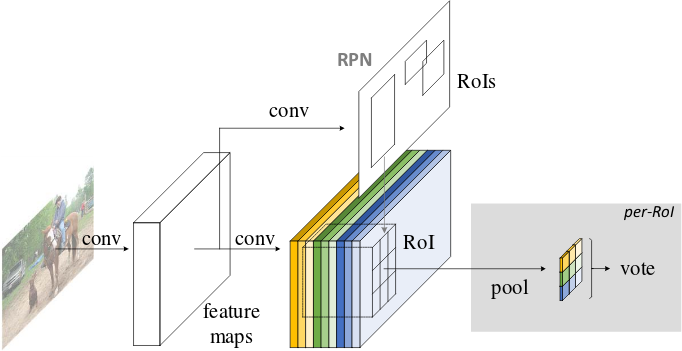
\includegraphics[width=0.8\columnwidth]{Figs/rfcnarchi.png}
      \caption{Architecture of \gls{rfcn}. Region proposals are found using the \gls{rpn} followed by classification based on a bank of position-sensitive score maps \cite{rfcn}.}
    \label{fig:rfcnarch}
\end{figure}

The added translation variance post finding proposals with the \gls{rpn} is done by producing a bank of $k^2$ score maps for each object category. Therefore, there are a total of $k^2(C + 1)$ maps. The number of $k^2$ maps is due to a $k \times k$ spatial grid representing relative positions. Typically $k = 3$, therefore, nine score maps represent position-sensitive scores for a given object category. This is illustrated in \figref{scoremaps}, each of the 9 coloured rectangles on the left of the figure represent the $k^2$ score maps. Each colour represents one of the relative positions. For example, the three shades of blue are positions in the bottom of a \gls{roi}, where the darkest is bottom-right, then bottom-centre and lightest bottom-right. For a given \gls{roi} placement the vote for relative position is sampled from their respective map in the bank.

\begin{figure}[H]
  \centering
    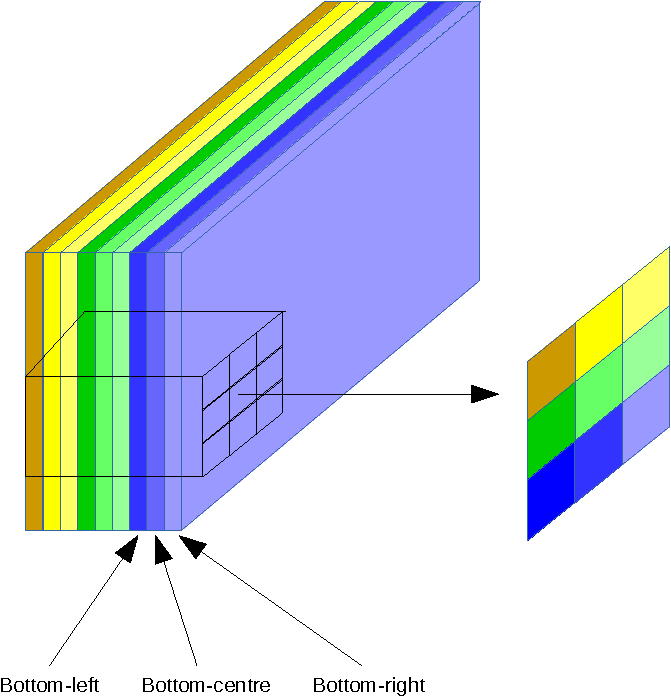
\includegraphics[width=0.4\columnwidth]{Figs/scoremaps1-crop.pdf}
     \caption{A bank of score maps are present for each object category. For a given \gls{roi}, the score is sampled from the respective position in the corresponding score map.}
    \label{fig:scoremaps}
\end{figure}

Once the bank of score maps have been computed, position-sensitive \gls{roi}-pooling is found for region classification. Each individual $k \times k$ bin pools from its corresponding location in the relevant score map. For example, the top left bin pools from that position in the top-left score map and so on. The \gls{roi}-pool is computed using average pooling for each bin which can be seen in \figref{rfcnpooling}. The final decision for a given class is determined by a vote where each of the bins are averaged, producing a $(C+1)$-dimensional vector for each \gls{roi}.

\begin{figure}[H]
  \centering
    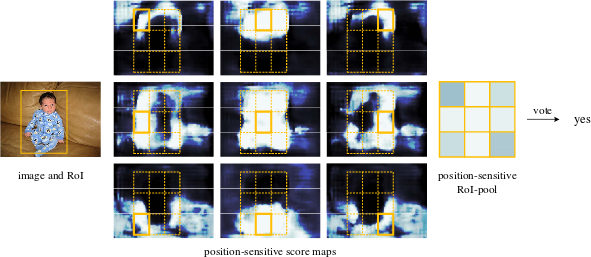
\includegraphics[width=1.0\columnwidth]{Figs/rfcnpooling.png}
      \caption{Position-sensitive \gls{roi}-pooling operation for a given class \cite{rfcn}.}
    \label{fig:rfcnpooling}
\end{figure}

\section{\uppercase{Proposed Method}}
Now that an analysis of the technical aspects of object detection with deep learning has been conducted an overview of the design of the system will be made in this section. 
Multiple choices can be made with respect to the overall architecture of the \gls{cnn}-based object detector. As covered in \sectionref{objdet}, two of the best performing systems are Faster R-CNN and R-FCN. The current core classification model used in both is the ResNet architecture. As the addition of ResNets significantly increases performance the use of these in this work is deemed crucial. However, the choice of either Faster R-CNN or R-FCN is not immediately as clear. Both methods perform similarly with respect to benchmarks such as \gls{pascalvoc} and \gls{mscoco}. But as the decision has been made to incorporate ResNets a decision on this matter was indirectly made. The GPU available in this project while being large in regards to memory is only available to train R-FCN with the ResNet-101 model. Unfortunately, due to the internal architecture of Faster R-CNN the 8GB memory on the NVIDIA GPU was not able to store all parameters while training a Faster R-CNN with ResNets. Due to the more efficient classification module in R-FCN, a ResNet backbone could be trained.
\\\\
Leading object detection systems take advantage of ensemble methods. Many of them are trained with regards to the variations in internal architecture and not specifically training experts towards solving specific challenges. Therefore, the system in this project will take advantage of the first point in \sectionref{build_ensemble}, namely data sampling and selection. The aim will be to train R-FCN with ResNet-101 on different subsets of training data with the aim to create expert ensemble members in regards robust-related challenges. Two separate factors will be chosen, one with respect to variations in the object and the other in terms of image variations. The first factor chosen is object size. As covered in \sectionref{benchresults}, in general object detection systems find it challenging to detect and classify objects with smaller resolutions. Therefore, if a system can be trained towards a subset of sizes in the training data, ideally the individual ensemble members will increase their performance on the respective sizes. The second factor chosen is image quality. As mentioned in \sectionref{probchallenges}, the quality of an image can be a factor in the overall performance of \gls{cnn}-based classification systems. Therefore members will also be trained towards subsets data split based upon this.
\\\\
Lastly, the third strategy in building an ensemble system will be addressed. Individual members predictions much be combined in an ensemble system. Therefore, approaches must be taken to combine outputs. The combination strategy is greater than only voting on which class a potential object is associated to. Bounding-boxes and the confidence of each detection is used in the calculation of metrics in both \gls{pascalvoc} and \gls{mscoco}. Therefore, these must be combined in the ensemble system as well.
\\\\
Based upon these issues the following design requirements are set with respect to the previously discussed items.

\begin{itemize}
	
	\item Object Detector Architecture.
	\begin{itemize}
		\item \gls{cnn}-based method.
		\item ResNets as backbone model.
	\end{itemize}

	\item Ensemble Data Sampling and Selection.
	\begin{itemize}
		\item Ability to measure object and image variations with respect to: 
		\begin{itemize}
			\item Object size.
			\item Image quality.
		\end{itemize}
	\end{itemize}

	\item Ensemble Training of Classifiers.
	\begin{itemize}
		\item Must be kept constant to measure effect of differing data sampling strategy.
	\end{itemize}

	\item Ensemble Combination.
	\begin{itemize}
		\item Method to combine bounding-boxes and confidences between individual ensemble members.
	\end{itemize}
\end{itemize}

Now that the general requirements have been outlined the following sections will cover the architectural considerations to ensure that the above requirements can be met.

\subsection{Training Ensemble Members}\label{sec:trainens}
The training of the R-FCN members will be done using \gls{caffe} \cite{caffe}. This was chosen due to the research being provided by the authors of R-FCN through training code and pre-trained \gls{caffe} models. However, as there is the requirement to combine detections between ensemble members, then the detections must be found based upon the same input to each model. One solution to this is to use the region proposals found using the \gls{rpn}. In a standard R-FCN the \gls{rpn} is an internal part of the network and is trained end-to-end. However, as these proposals must be constant between all ensemble members this method is not appropriate. Additionally, due to the nature of the \gls{caffe} framework, once a network has been defined and trained it is difficult to change it. For example, a standard R-FCN takes the entire image as inputs but in this work the requirement is that it takes smaller region proposals. The solution to these points is to train the networks using a method inspired by the 4-step alternating training method presented by the Faster R-CNN authors \cite{fasterrcnn}. The process can be seen in \figref{4steptrain}.

 \begin{figure*}[!h]
  \centering
    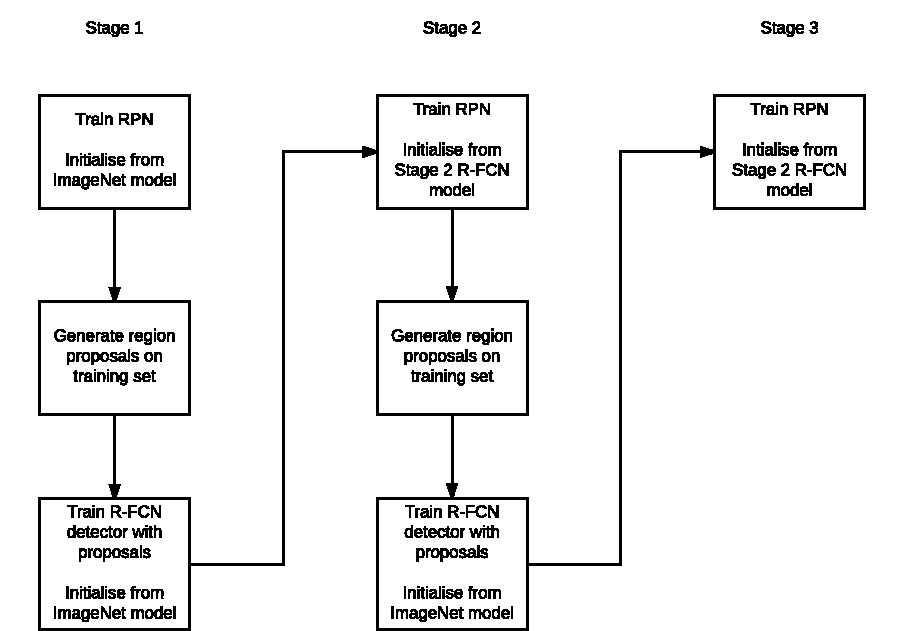
\includegraphics[width=1.8\columnwidth]{Figs/4step-crop.pdf}
      \caption{Flow chart showing the alternating training method.}
    \label{fig:4steptrain}
\end{figure*}

In this approach the overall network in trained in multiple steps rather than an end-to-end method. In the first step, an \gls{rpn} is trained to determine region proposals, the \gls{rpn} is initialised from a pre-trained ImageNet model and fine-tuned to the proposal task. Next a \gls{rfcn} is trained based upon the proposals found in the previous step. This network is also initialised with a pre-trained ImageNet model. In step three, another \gls{rpn} is trained but initialised using the \gls{rfcn} from step two. In this step the convolutional layers that are shared between the \gls{rfcn} and \gls{rpn} are fixed and only the layers unique to the \gls{rpn} are updated. By training a model with this approach a testing image is able to run through the same steps as a \gls{rfcn} trained end-to-end, however, as the networks are split into different models it is also possible to use the stages of the method individually. Creating a solution for finding region proposals with an external \gls{rpn} and having a \gls{rfcn} that can take the proposals as inputs. 
\\\\
An additional benefit to training \glspl{rfcn} in this manner is that once a baseline model has been created only one part needs to be re-trained. As the aim is to train various ensemble members to different subsets of data only the \gls{rfcn} in stage 2 is required to be re-purposed. The \gls{rpn} in stage 3 should be kept constant based on the baseline model as it will provide the shared proposals for test images. Therefore, once a systematic approach has been found for splitting data for both train and test based on the data sampling and selection requirements the detection part of the \gls{rfcn} can be trained towards its expert area. The following sections will explain how the subsets of data will be selected.

\subsubsection{Object Size Data Sampling}
The area of a region proposal found with a \gls{rpn} gives an indication as to the approximate size of a potential objects. Therefore, the area for all proposals on the training set can be computed from the output of the second step in stage 2 shown in \figref{4steptrain}. Once the area of all proposals are computed an appropriate split of the data can be determined depending on the area distribution. The main requirement in creating the subsets of data is that equal number of ground truth samples should be present in both.

\subsubsection{Image Quality Data Sampling}
There are many choices for computing the quality of an image. A popular area of research for this purpose is \gls{iqa}. These methods aim to determine the subjective quality of an image. There are two forms of \gls{iqa}, \gls{friqa} and \gls{nriqa}. \gls{friqa} approaches require the original, undistorted reference image in order to determine quality. Whereas, \gls{nriqa} do not have this information available \cite{deepiqa}. As the aim is to determine the level of image quality on one of the benchmark datasets, no reference image is present. Therefore, an \gls{nriqa} method is required. Current state-of-the-art within \gls{nriqa} is also deep learning based and works are typically trained on \gls{iqa} datasets. Datasets include \gls{live} dataset \cite{livepaper} \cite{liveweb}, TID2013 \cite{tid2013} and CSIQ \cite{csiq}. The datasets consist of source reference image and have artificially created counterparts with varying levels of distortion. Distortions include, such as in the LIVE dataset, JPEG2000 compression, JPEG compression, additive white Gaussian noise, Gaussian blur and bit errors from a fast fading Rayleigh channel. Models can then be trained to predict subjective quality based on ground truth user determined quality measurement.
\\\\
Based upon this, an \gls{nriqa} method can be used to determine the level of image quality with respect to a number of different distortions. Then as in object size training, if possible, the data will be split into different training subsets. A leading \gls{cnn}-based \gls{nriqa} method will be used and the specific network and implementation details will be covered in \sectionref{iqaimp}.

\subsubsection{\gls{rfcn} Training}
Training of the baseline \gls{rfcn} model shown in \figref{4steptrain} is done using \gls{sgd} optimisation with largely the same parameters across the five different training parts. The parameters are adapted from \cite{rfcn} and can be seen in \tableref{trainparams}. All models start with a base learning rate of 0.001 which is dropped by a factor of 0.1 once in the process. This is done after 80,000 iterations for the \gls{rfcn} models and after 60,000 for the \glspl{rpn}. The learning rate is controlled with a momentum of 0.9 and weight decay of 0.0005. The two \gls{rfcn} models are trained for 120,000 iterations, while the three \glspl{rpn} are trained for 80,000.

\begin{table}[h]
\centering
\caption{Common \gls{sgd} optimisation parameters for the 5 training parts of the baseline \gls{rfcn} model.}
\label{tab:trainparams}
\begin{tabular}{|l|l|}
\hline
\textbf{Parameter}            & \textbf{Value}  \\ \hline
Base learning rate   & 0.001  \\ \hline
Learning rate policy & step   \\ \hline
Gamma                & 0.1    \\ \hline
Momentum             & 0.9    \\ \hline
Weight decay         & 0.0005 \\ \hline
\end{tabular}
\end{table}

 Both networks are trained with a batchsize of one example per iteration. In the \gls{rpn} models the batches are simply one ground truth example per iteration. Whereas, the training of the \glspl{rfcn} sample 128 mini-batches from a given image. These mini-batches can consist of both object class samples and background samples. 
 The only data augmentation used in training is horizontal flipping of images, effectively creating double the amount of training examples.

 \subsection{Object Detection Benchmark}
 The choice of object detection benchmark is \gls{pascalvoc}. A common strategy in object detection systems is the conduct preliminary experiments on \gls{pascalvoc} data. Then if applicable a potential system can be trained on a larger dataset such as \gls{mscoco}. By training on \gls{pascalvoc} a larger number of ensemble members can be trained on the single GPU available.
 \\\\
 The data used will follow the leading methods for \gls{pascalvoc} 2007 object detection. Training will be done on the 07+12 train sets and testing will be conducted on the 07 test set.

\subsection{Resolution-Aware Detection}
As determined earlier object detectors are generally more accurate on objects that cover a larger number of pixels in an image. This is intuitive as objects with a lower resolution objectively have less details that can describe them. The poorer performance can be seen in \tableref{cocores}, for all object detectors the \gls{ap} is considerably lower for smaller objects in comparison to both medium and large. The best performing detector from \cite{deepres}, has an \gls{ap} difference of 35.3\%, from 50.9\% for large objects to 15.6\% for small. 
A potential method of tackling this issue is to train multiple detectors on separate partitions of the training data according to the size of the object. While deep-based \gls{cnn} have millions of parameters to generalise from training to testing, the difference between small and large objects may skew the learning towards the latter. In order to test this hypothesis an initial test will be conducted on the 07+12 train set. However, \gls{pascalvoc} does not have the same definition of objects sizes as in \gls{mscoco}. Therefore, the distribution of the ground truth bounding boxes from the 07+12 set must be analysed in order to determine if an appropriate split of data based on object size can be made. This was done by parsing all of the bounding box coordinates in the set and calculating the area. A histogram of the all of the ground truth areas can be seen in \figref{0712hist}. There is a clear tendency to smaller objects in the training set with a clear skew towards the left of the figure.

\begin{figure}[H]
  \centering
    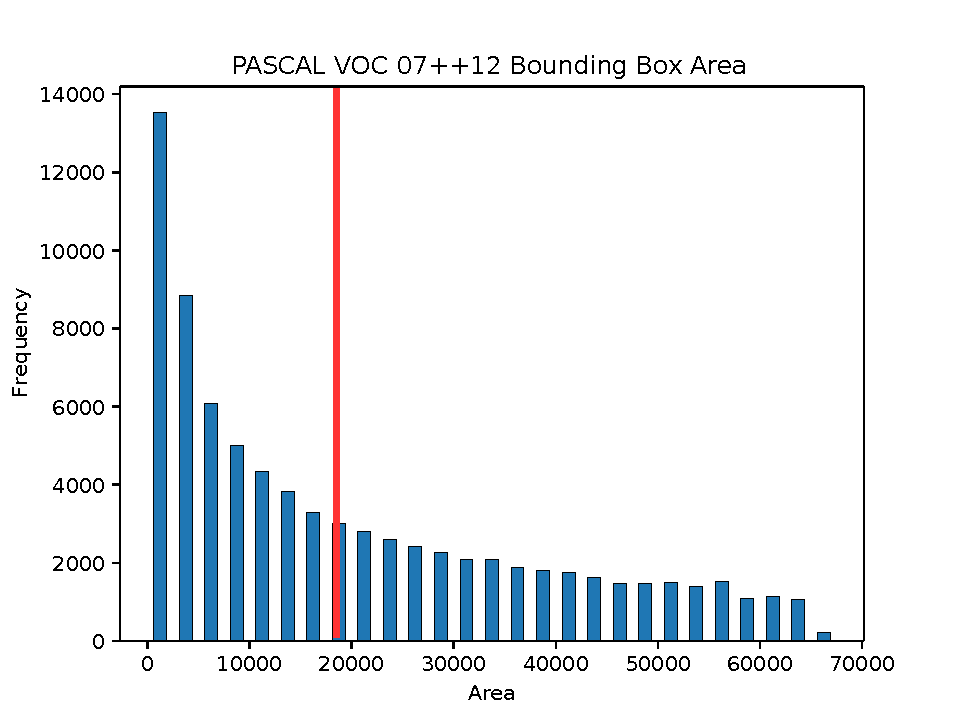
\includegraphics[width=0.6\columnwidth]{Figs/0712histred.pdf}
      \caption{Histogram of the \gls{pascalvoc} 07+12 bounding box area.}
    \label{fig:0712hist}
\end{figure}

The data in \figref{0712hist} can be split into two equal subsets if the median area of 19,205.5 is used. However, the ensemble \gls{rfcn} members are trained with region proposal inputs of both ground truth positives and negative examples found using a \gls{rpn}.

A potential shortcoming of using proposals as inputs to training ensemble members is a \gls{rpn} likely finds many more examples of possible objects than actually are present. For a given image, an \gls{rpn} may find hundreds of potential objects despite an image only containing a couple of true positive examples. This can be solved by setting the proposals with the highest confidence as the ground truth examples and labelling the remaining proposals as the background class. This is a stark comparison to the end-to-end training approach as there are now many more training examples and a large skew towards the background class. With this approach, the total number of training examples is increased from 80,116 ground truth object instances to 9,979,345 region proposals. The median of the almost 10 million proposals is 4,684 pixels, significantly smaller than the threshold of 19,205.5 determined using only ground truth boxes. This large increase in training examples and skew in data poses a question on how to split the \gls{rpn} proposals such that two networks can be trained towards small and large objects equally. As mentioned earlier, a pre-requisite in creating subsets of data is that the multiple sets should be roughly equal in regards to ground truth examples. If the subsets were split by the median of the \gls{rpn} proposals (4,684) the two sets of data would have equal numbers of examples. However, the large skew in \gls{rpn} proposals to smaller objects means that there significantly more ground truth samples in the subset of data containing larger objects. This can be seen in \tableref{splitrpn}, where despite there being an almost even split in data subsets there are significantly more ground truth annotations in the \gls{rpn}$_{larger}$ subset.

\begin{table}[h]
\centering
\caption{Creating object resolution data subsets. If split by the median area of all region proposals training samples the larger dataset has significantly more ground truth object instance samples.}
\label{tab:splitrpn}
\begin{tabular}{|l|l|l|}
\hline
\textbf{Data} & \textbf{RPN$_{small}$} & \textbf{RPN$_{larger}$} \\ \hline
Ground Truth & 19,992    & 60,116     \\ 
Background   & 4,969,369 & 4,929,297  \\ \hline
Total        & 4,989,361 & 4,989,413  \\ \hline
\end{tabular}
\end{table}

Another option is to use the median of 19,205.5 found on only ground truth boxes. The data distribution based on this threshold can be seen in \tableref{splitgt}. In this instance there is significantly more data in the \gls{rpn}$_{larger}$ subset, however, the skew is solely due to the many more background examples. The ground truth annotations are shared equally with 40,058 samples in each.

\begin{table}[h]
\centering
\caption{Creating object resolution data subsets. If split by the median of area from ground truth objects there is an equal number of ground truth instances. However, \gls{rpn}$_larger$ has significantly more background samples.}
\label{tab:splitgt}
\begin{tabular}{|l|l|l|}
\hline
\textbf{Data} & \textbf{RPN$_{small}$} & \textbf{RPN$_{larger}$} \\ \hline
Ground Truth & 40,058    & 40,058     \\ 
Background   & 3,528,370 & 6,370,859  \\ \hline
Total        & 3,568,428 & 6,410,917  \\ \hline
\end{tabular}
\end{table}

As the overall goal of object detectors is to find objects within the classes, the decision was made to use the threshold of 19,205.5 to create the split in data. Despite there being significantly more background examples in one of the datasets. 
\\\\
\gls{rfcn} ensemble members were trained on the two subsets of \gls{rpn} according to the design guidelines. To evaluate how well the expert resolution members perform on the respective subsets of data tests were performed on splits of the 07 test data. This data was split by using the same median threshold of 19,205.5 used in creating the training subsets. Firstly, the results for small objects from 07 test can be seen in \tableref{small07res}. Shown are \glspl{rfcn} trained on \gls{rpn}$_{small}$, \gls{rpn}$_{larger}$ and a baseline model trained on all 07+12 data. The shows that the model trained towards smaller object proposals on \gls{rpn}$_{small}$ performs best. This trend is similarly true for large objects as seen in \tableref{large07res}. Finally, for all ground truth objects the baseline model is the best performing as seen in \tableref{alldatares}.


\begin{table}[h]
\centering
\caption{Results for \gls{rfcn} models trained on three different subsets of data and tested on only small objects from the 07 test set.}
\label{tab:small07res}
\begin{tabular}{|l|l|}
\hline
\textbf{Train Data} & \textbf{\gls{ap}}      \\ \hline
\gls{rpn}$_{small}$      & \textbf{55.00\%} \\ \hline
\gls{rpn}$_{larger}$      & 20.92\% \\ \hline
07+12        & 43.80\% \\ \hline
\end{tabular}
\end{table}

\begin{table}[h]
\centering
\caption{Results for \gls{rfcn} models trained on three different subsets of data and tested on only large objects from the 07 test set.}
\label{tab:large07res}
\begin{tabular}{|l|l|}
\hline
\textbf{Train Data} & \textbf{\gls{ap}}      \\ \hline
\gls{rpn}$_{small}$      & 21.28\% \\ \hline
\gls{rpn}$_{larger}$      & \textbf{81.81\%} \\ \hline
07+12        & 75.14\% \\ \hline
\end{tabular}
\end{table}


\begin{table}[h]
\centering
\caption{Results for \gls{rfcn} models trained on three different subsets of data and tested on all of the 07 test set.}
\label{tab:alldatares}
\begin{tabular}{|l|l|}
\hline
\textbf{Train Data} & \textbf{\gls{ap}}      \\ \hline
\gls{rpn}$_{small}$      & 46.74\% \\ \hline
\gls{rpn}$_{larger}$      & 62.48\% \\ \hline
07+12        & \textbf{79.59\%} \\ \hline
\end{tabular}
\end{table}

Based upon these results it was determined that the ensemble member experts towards object size was suitable. The following section will explain the data sampling and training for image quality ensemble members.


\subsection{IQA Detection}
To evaluate the amount of distortions in the dataset a method for \gls{iqa} is needed. A recent state of the art method is that of deep IQA \cite{deepiqa}. Deep IQA is a \gls{cnn}-based \gls{nr} \gls{iqa} method that can be trained to measure the subjective visual quality of an image. It is deeper than previous \gls{cnn}-based \gls{iqa} methods with the architecture being inspired by VGG nets \cite{vgg16}. Deep IQA consists of 14 convolutional layers, 5 max-pooling layers and 2 fully-connected layers. The architecture is shown in \figref{deepiqa_arch}. The convolutional layers are all 3$\times$3 convolution kernels and activated using \gls{relu}. Inputs to each convolutional layer are zero-padded to ensure output size is equal to the input. Max-pooling layers consist of 2 $\times$ 2 sized kernels. The network is trained on mini-batches of 32 $\times$ 32 patches. During inference non-overlapping patches are sampled from the image and image quality scores are predicted for each instance. The patch scores are averaged for the final score for the entire image. 

\begin{figure}[H]
  \centering
    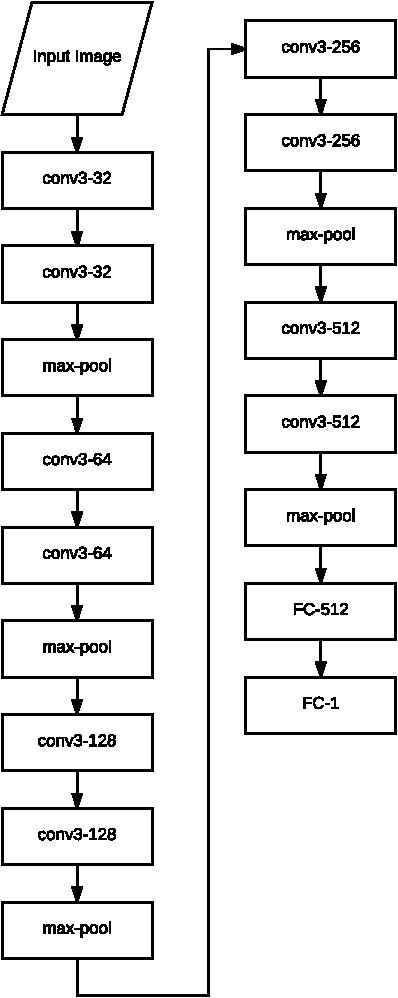
\includegraphics[width=0.3\columnwidth]{Figs/deepiqa_arch.pdf}
      \caption{Architecture of the deep IQA network. Notation for convolutional layers are conv(receptive field size)-(number of channels) and fully-connected layers are FC(number of channels).}
    \label{fig:deepiqa_arch}
\end{figure}

Training deep IQA requires a database of annotated images with both reference images and distorted counterparts. The following section will outline the database used in this project for \gls{iqa} training.

\subsection{LIVE Image Quality Database}
Deep IQA assesses three different datasets for this purpose. These are \gls{live} which consists of 5 different distortions \cite{livepaper}, TID2013 \cite{tid2013} with 24 different distortions and CSIQ \cite{csiq} with 5 types. For simplicity purposes the only \gls{live} dataset is chosen for this project. The dataset was made for the purposes of evaluating the subjective visual quality of images in regards to the five distortion types. The distortions are generated from 29 colour reference images that are of both high-resolution and high quality. An example of images from the dataset can be seen in \figref{live_ex}. The references image were collected to have a wide variety in different content, this includes faces, people, animals, nature and man-made objects.

The five distortions generated from the reference images are Gaussian blur, white noise, JPEG compression, JPEG2K compression and fast fading. By varying the parameters used in creation of the distortions a larger database is created for each type. The total number of images is 982 where 174 are for Gaussian blur, white noise and fast fading. JPEG and JP2K compression have 233 and 227 images respectively. The distorted images were created as follows:

\begin{itemize}
	\item Gaussian blur: blur is added to the images using a circular-symmetric Gaussian kernel of standard deviation $\sigma_B$. The values of $\sigma_b$ are sampled between the range of 0.42 to 15 pixels.
	\item White noise: Gaussian white noise of standard deviation $\sigma_N$ is added to all RGB pixels. Firstly, pixel values are scaled to between 0 and 1. $\sigma_N$ varying between 0.012 and 2.0 is added, afterwards pixel values are rescaled back between 0 and 255.
	\item JPEG compression: compression artefacts are added to the reference bitmap images with JPEG at bit rates between 0.15 \gls{bpp} to 3.34 \gls{bpp}.
	\item JP2K compression: artefacts added ranging between 0.028 \gls{bpp} to 3.15 \gls{bpp}.
	\item Fast fading: this distortion represents errors that can occur when a JP2K bitstream is transmitted over a wireless channel. The receiver signal-to-noise-ratio is varied between 15.5 to 26.1dB for bit errors.
\end{itemize}

Subjective image quality values were calculated by showing human subjects all images, including reference images, and asking them to rate the image as either bad, poor, fair, good, or excellent. The rating was done using a slider on a graphical interface with the five possibilities being evenly spaced. A value between [1, 100] was then found depending on where the subject paced their rating. \gls{dmos} were calculated for each image and averaged between all users for the final image quality annotation for an image. A low \gls{dmos} represents high image quality and a high \gls{dmos} is a low quality image. \figref{gb_ex} shows an example of an image with four varying levels of Gaussian blur and their \gls{dmos} values.

\begin{figure*}[!h]
\minipage{0.2\textwidth}
  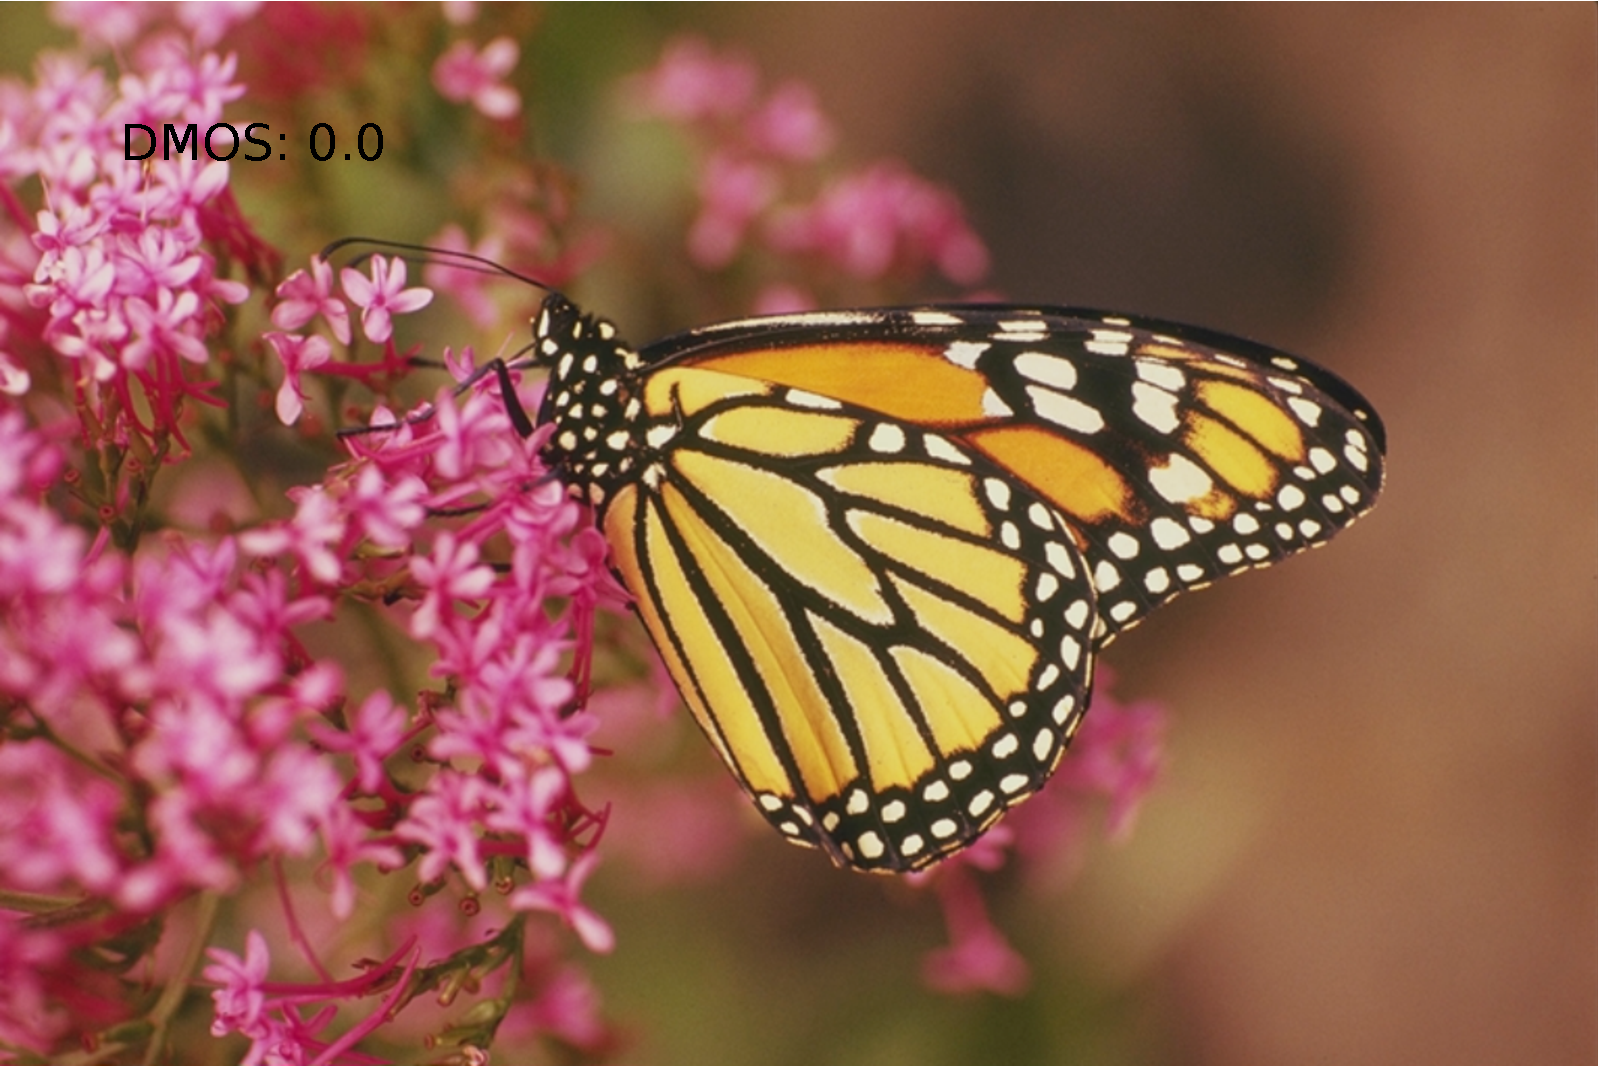
\includegraphics[width=\linewidth]{Figs/img173.pdf}
  \caption*{\gls{dmos}: 0.0}\label{fig:}
\endminipage\hfill
\minipage{0.2\textwidth}
  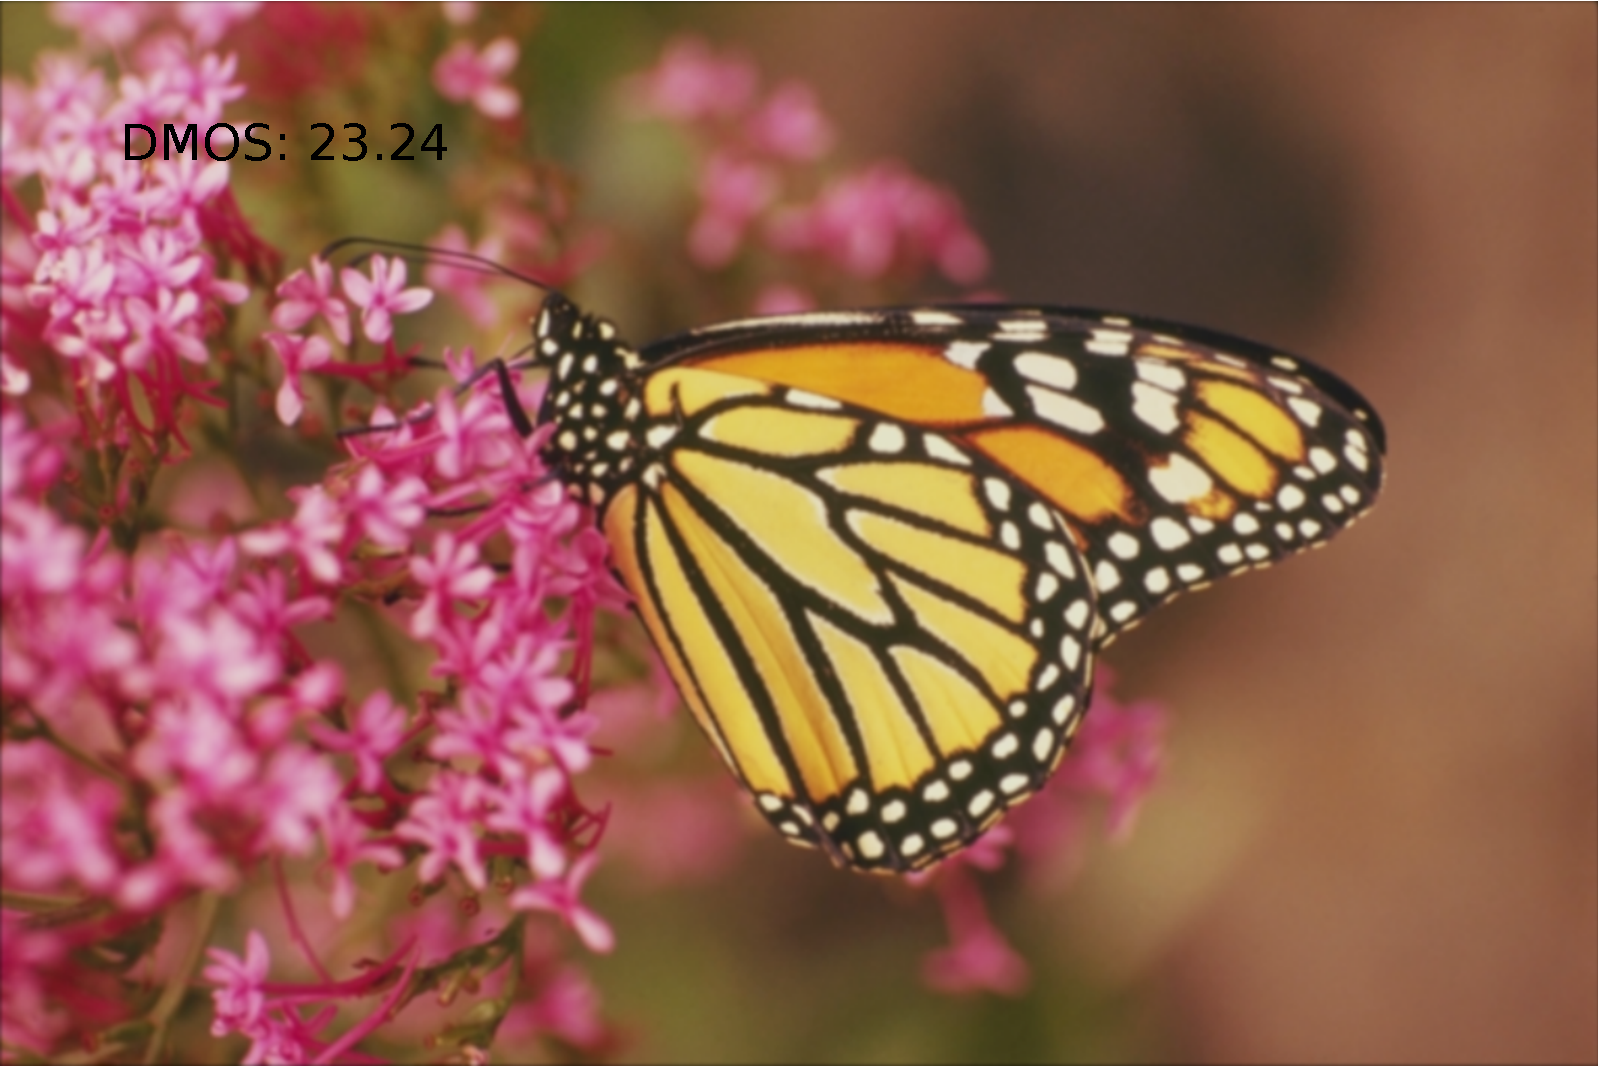
\includegraphics[width=\linewidth]{Figs/img96.pdf}
  \caption*{\gls{dmos}: 23.24}\label{fig:}
\endminipage\hfill
\minipage{0.2\textwidth}
  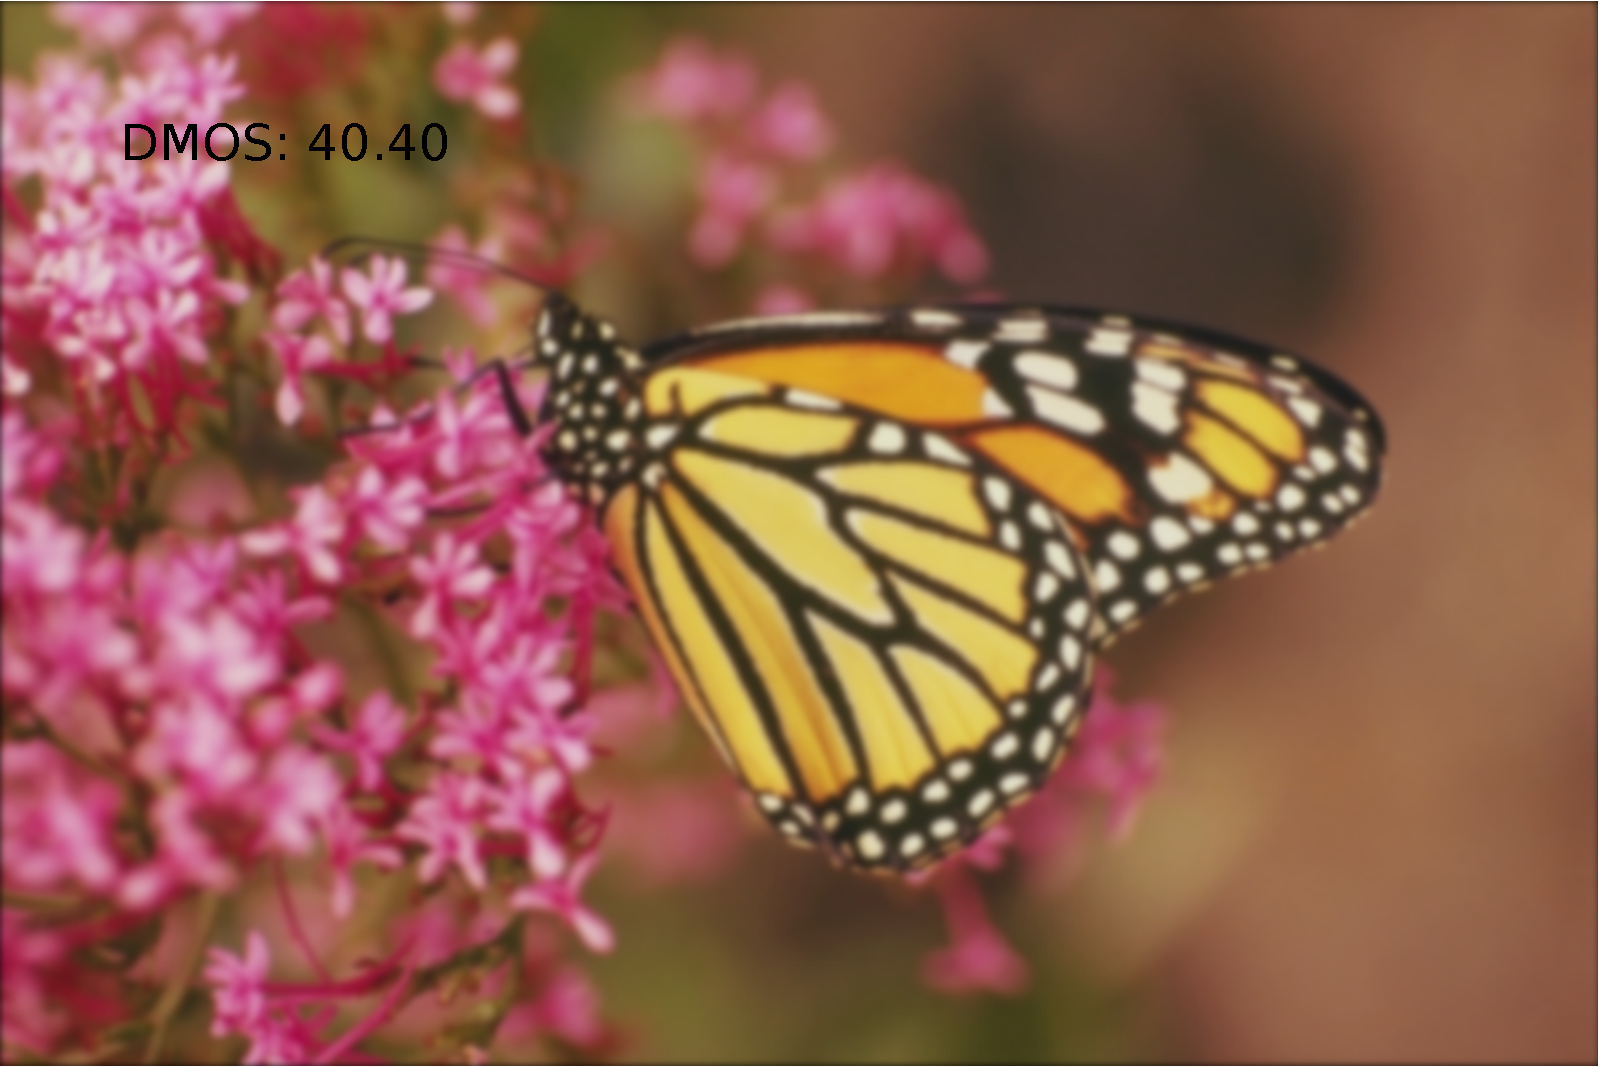
\includegraphics[width=\linewidth]{Figs/img103.pdf}
  \caption*{\gls{dmos}: 40.40}\label{fig:}
\endminipage\hfill
\minipage{0.2\textwidth}
  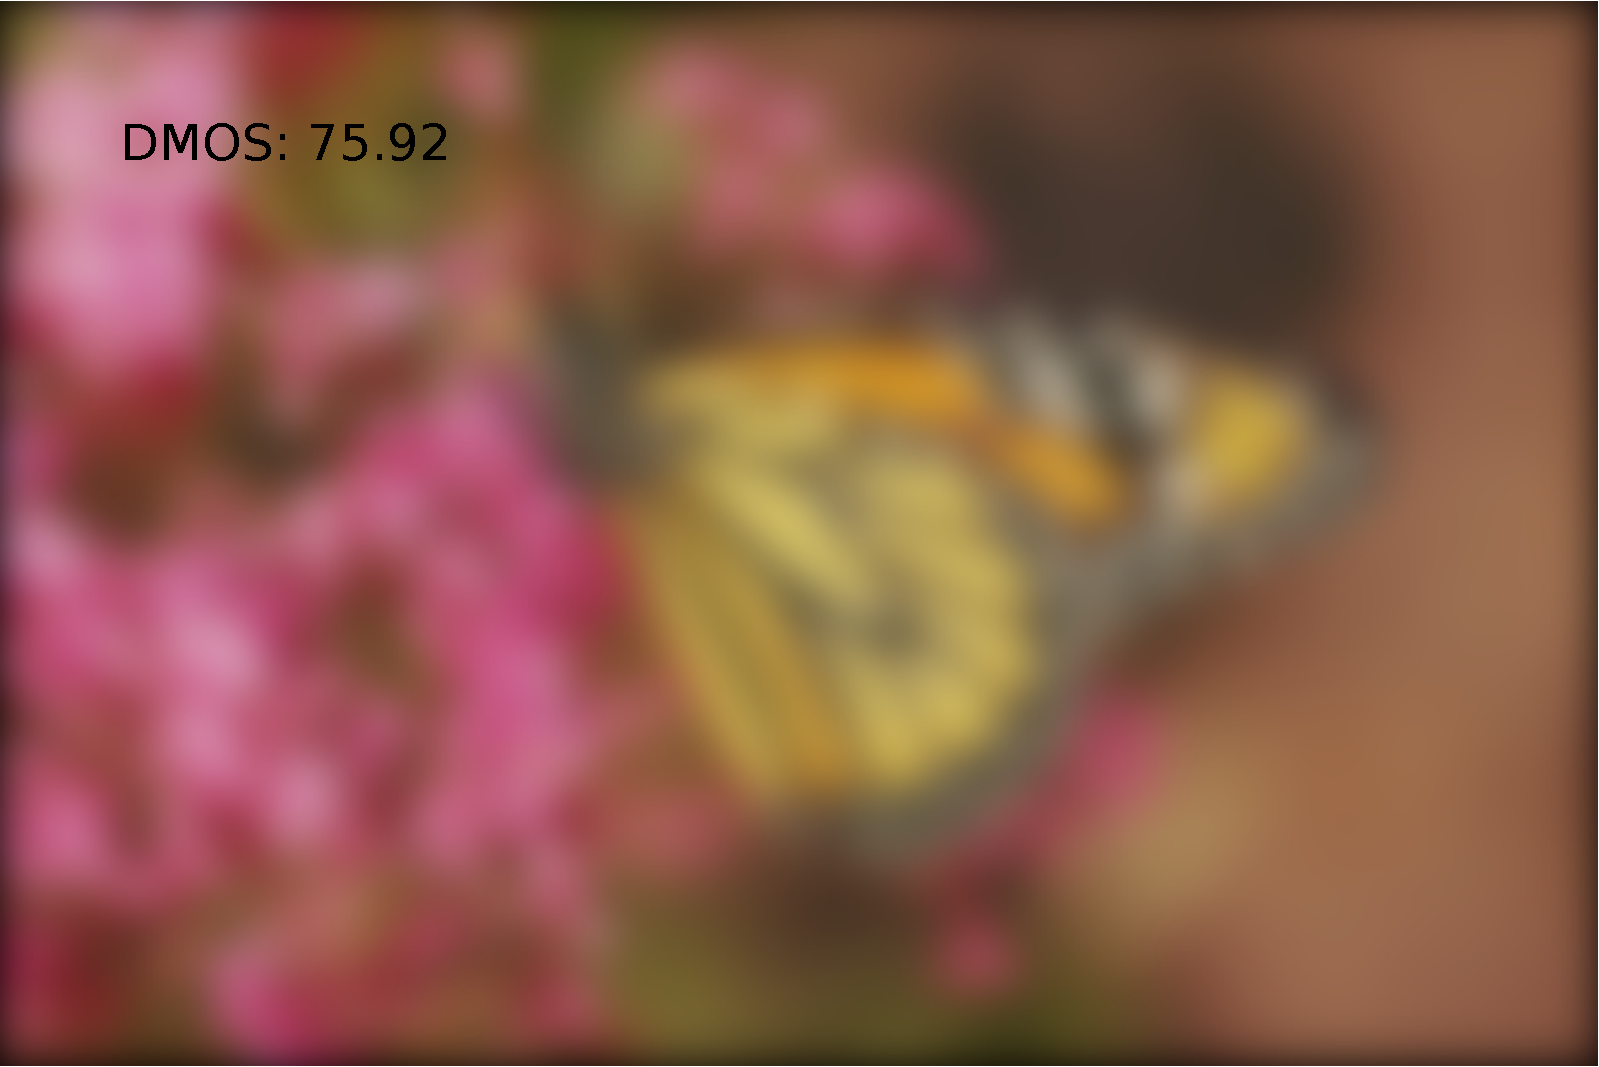
\includegraphics[width=\linewidth]{Figs/img11.pdf}
  \caption*{\gls{dmos}: 75.92}\label{fig:}
\endminipage\hfill
\caption{Four example images from the Gaussian blur distortion set. Respective \gls{dmos} scores are shown on the image and below.}
\label{fig:iqdist}
\end{figure*}

Given the annotated \gls{dmos} values a system can be trained to predict the image quality of an image. The following section will outline how to train deep IQA for this purpose.

\subsection{Training Deep IQA}
In the original work the deep IQA model \cite{deepiqa} is trained for all five distortion types present in \gls{live} \cite{livepaper} \cite{liveweb}. While this can provide insights into general image quality, individual models are needed to create a potentially more powerful ensemble. The \gls{nriqa} model was provided by the authors and by taking advantage of the fine-tuning technique, models for each of the individual distortions can be trained in a timely manner. The model was provided for the Chainer framework \cite{chainer} and fine-tuning of individual models were done using this. Fine-tuning takes a previously trained model and uses these parameters as a starting point, rather than other commonly used initialisation techniques such as using a Gaussian distribution. As the model is already trained towards all distortions the assumption can be made that only a shorter training cycle is necessary to the new task. The five fine-tuned models are trained in a similar manner to that of the provided model following the guidelines in the original work \cite{deepiqa}. 
\\\\
In the \gls{live} dataset there are 29 reference images from where the respective distortions have been created. When training deep IQA, the reference images are randomly split into 17 training images, 6 validation images and 6 test images. The deep IQA models are trained using mini-batches consisting of a total of 128 patches per forward/backward pass. The patches are sampled from four randomly selected images from the training split and each image accounts for 32 of the 128 patches in the mini-batch. This process is continued until no more patches are available for mini-batch sampling. This constitutes a completed epoch and all patches are again available for the next epoch. The model provided by the authors was trained for 3,000 epochs, however, as mentioned fine-tuning can drastically reduce the number of epochs required. Therefore, the models for the five distortions are trained for only 500 epochs each. The optimisation method for parameter updates is Adam \cite{adam}. The optimisation settings for Adam are unchanged to that of those used in training the original model. They are as $\beta_1$ = 0.9, $\beta_2$ = 0.999, $\epsilon$ = 10$^{-8}$ and $\alpha$ = 10$^{-4}$. A total of 10 models are trained for each distortion type, each on their individual random split of the 29 reference images. After each of the 500 epochs the model is evaluated on the validation set and the epoch with the best performance is chosen as the final model for testing. The evaluation metrics used for both the validation and test set is \gls{lcc} and \gls{srocc}. \gls{lcc} is used for prediction accuracy as it is a measure of the linear correlation between two sets of data. \gls{srocc} evaluates the prediction monotonicity by measuring the rank correlation between the two sets. For both metrics a value of +1 indicates a positive correlation, 0 is no correlation, and -1 is a negative correlation.
\\\\
The mean results for each of the distortion types from their 10 models can be seen in \tableref{iqaavg}. Each best performing model on the respective validation sets are run on the testing sets and averaged. The results showed that well-performing deep IQA models were successfully trained towards the individual distortion types. The following section will cover how the \gls{pascalvoc} data will be split in subsets based upon these deep IQA models.

\begin{table}[h]
\centering
\caption{Average results from 10 trained deep IQA models for each distortion type.}
\label{tab:iqaavg}
\begin{tabular}{|l|l|l|}
\hline
\textbf{Distortion Type} & \textbf{\gls{lcc}}    & \textbf{\gls{srocc}}  \\ \hline
Gaussian Blur   & 0.9750 & 0.9681 \\ \hline
White Noise     & 0.9957 & 0.9887 \\ \hline
JPEG            & 0.9805 & 0.9523 \\ \hline
JP2K            & 0.9788 & 0.9600 \\ \hline
FF     & 0.9679 & 0.9505 \\ \hline
\end{tabular}
\end{table}


\subsection{PASCAL VOC Data Split}
Each model for the five distortion types and run through the 07+12 dataset in order to give an indication to the respective distributions, as done for the object sizes in \sectionref{resawareSec}. The distributions can been seen in the histograms in \figref{iqdist}.

\begin{figure*}[!h]
\minipage{0.2\textwidth}
  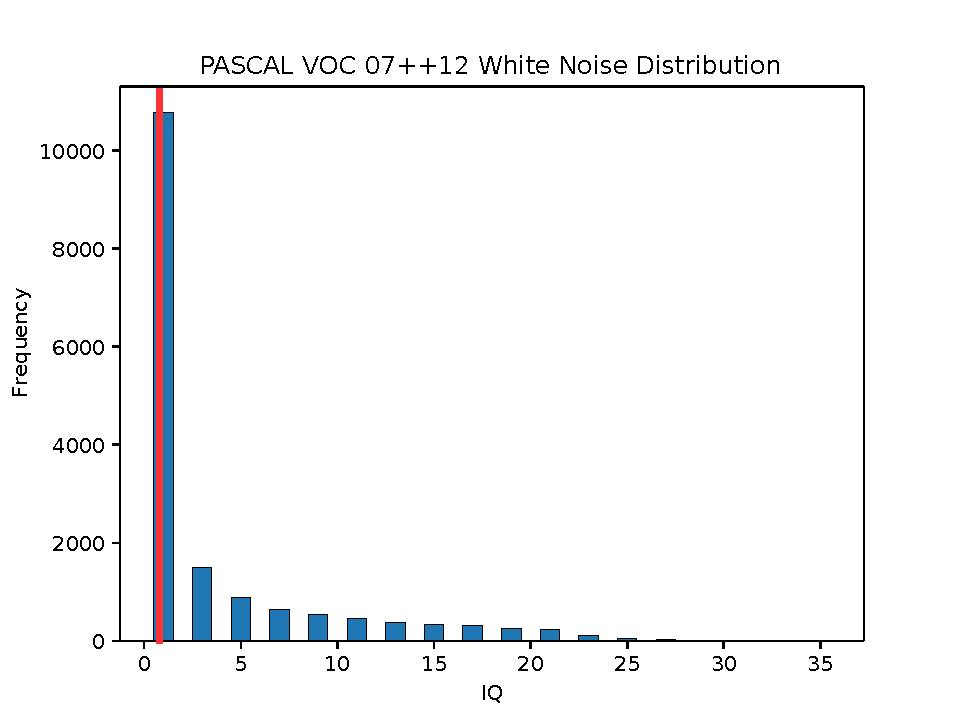
\includegraphics[width=\linewidth]{Figs/WhiteNoisedistred.pdf}
  \caption*{}\label{fig:}
\endminipage\hfill
\minipage{0.2\textwidth}
  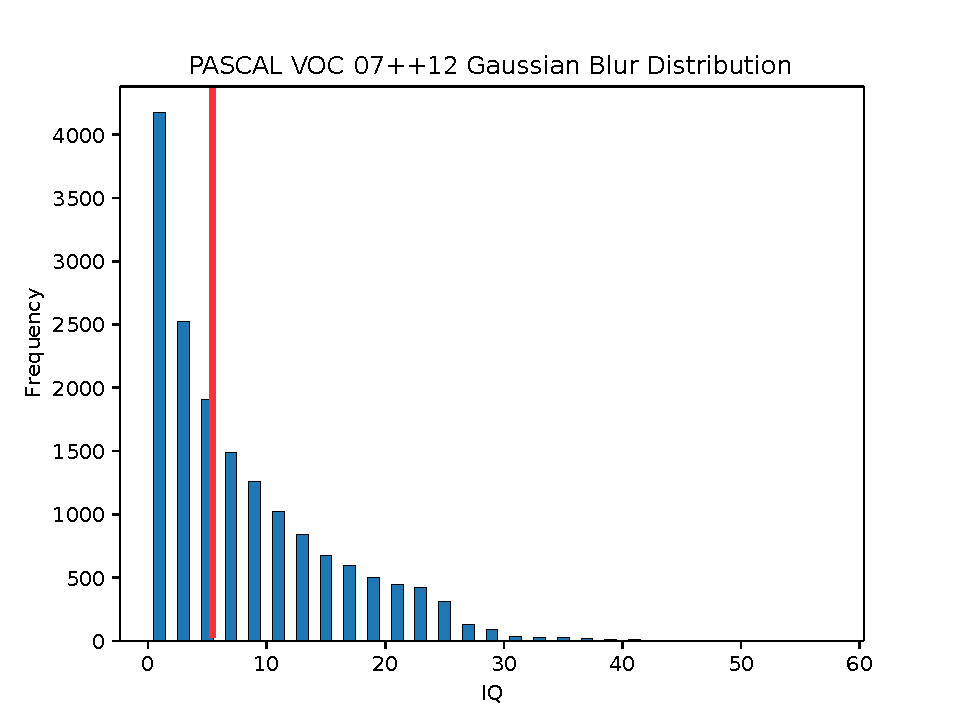
\includegraphics[width=\linewidth]{Figs/GaussianBlurdistred.pdf}
  \caption*{}\label{fig:}
\endminipage\hfill
\minipage{0.2\textwidth}
  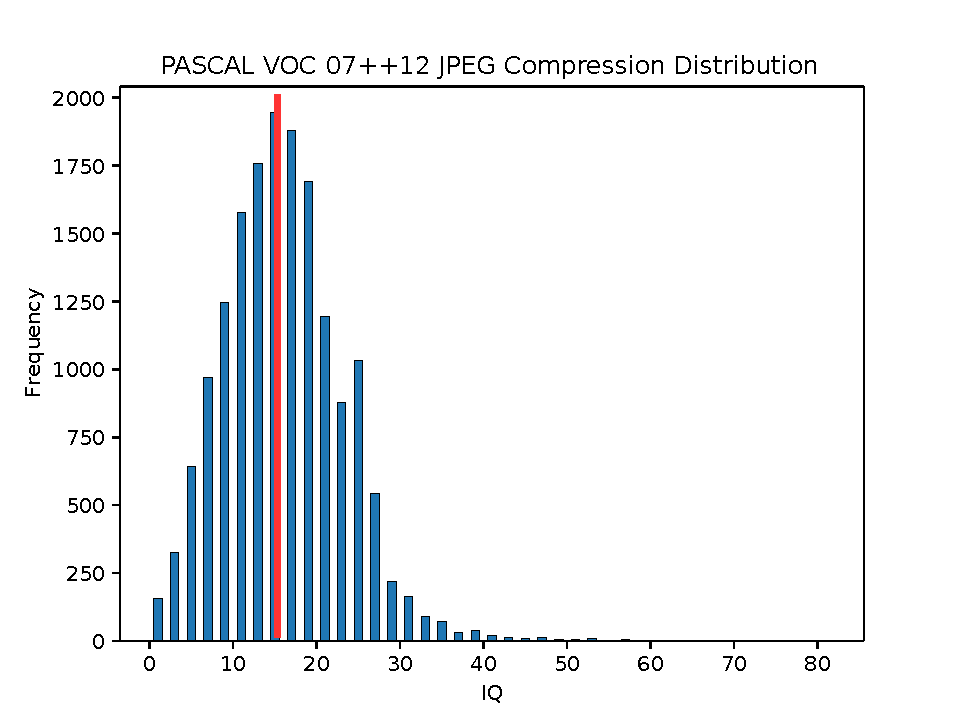
\includegraphics[width=\linewidth]{Figs/JPEGCompressiondistred.pdf}
  \caption*{}\label{fig:}
\endminipage\hfill
\minipage{0.2\textwidth}
  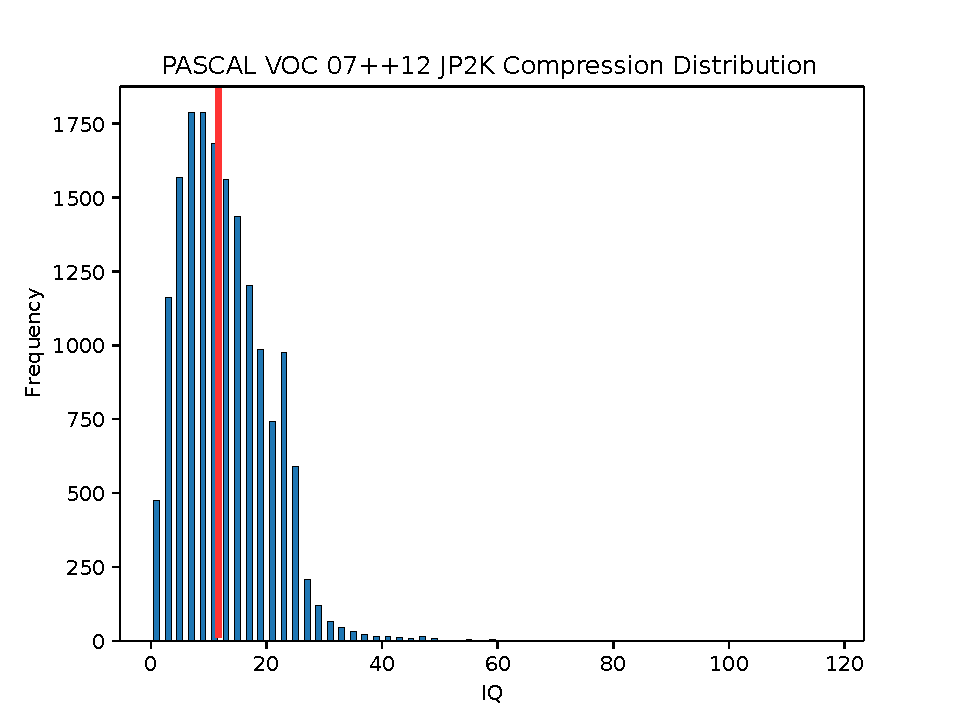
\includegraphics[width=\linewidth]{Figs/JP2KCompressiondistred.pdf}
  \caption*{}\label{fig:}
\endminipage\hfill
\minipage{0.2\textwidth}%
  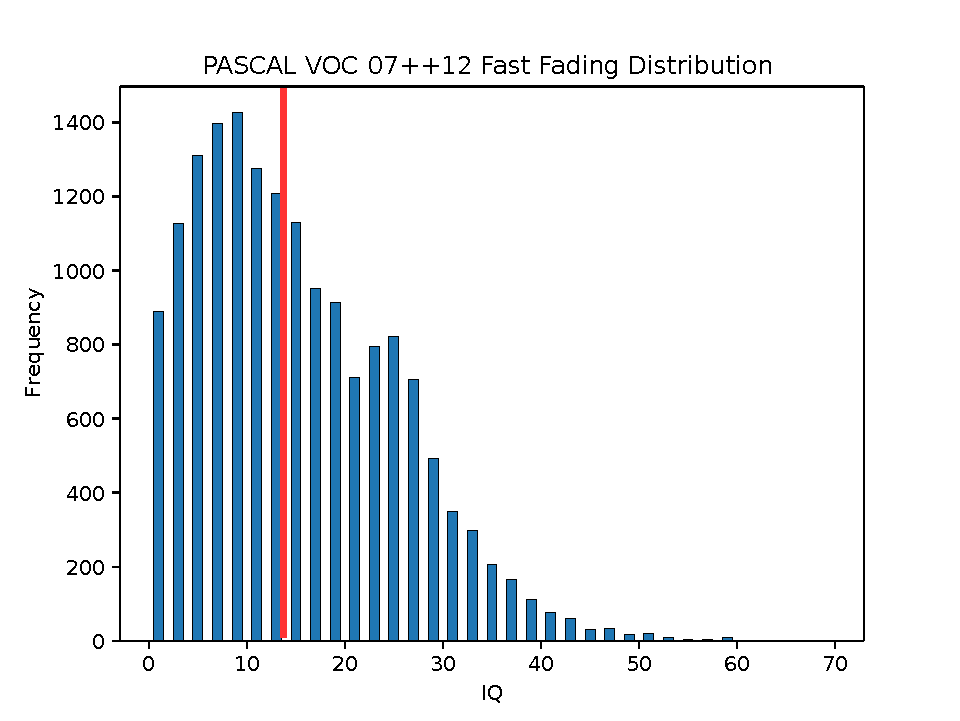
\includegraphics[width=\linewidth]{Figs/FastFadingdistred.pdf}
  \caption*{}\label{fig:}
\endminipage
\caption{Histograms representing the distribution of image quality for the five distortions trained from the \gls{live} image quality dataset. The distortions shown are white noise (a), Gaussian blur (b), JPEG compression (c), JP2k compression (d), fast fading (e).}
\label{fig:iqdist}
\end{figure*}

The distribution for white noise and Gaussian blur is skewed towards a higher image quality as seen in \figref{dist_wn} and \figref{dist_gb} and also to a lesser extent in fast fading in \figref{dist_ff}. Whereas the image quality for compression distortions is somewhat of a Gaussian nature in \figref{dist_jp} and \figref{dist_jk}. For determining an appropriate manner to split the data the same constraints are made as in that for object sizes, namely that both subsets of data should have an equal number of ground truths to train on. Again by taking the median for each of the five distributions can satisfy this. The respective medians can be seen in \tableref{iq_splits}.

\begin{table}[h]
\centering
\caption{Threshold values used for each distortion type to create even subsets of training data from 07+12.}
\label{tab:iq_splits}
\begin{tabular}{|l|l|}
\hline
\textbf{Distortion Type}   & \textbf{Median} \\ \hline
White Noise       & 0.599  \\ \hline
Gaussian Blur     & 5.607  \\ \hline
JPEG Compression  & 15.660 \\ \hline
JP2K Compression & 11.747 \\ \hline
Fast Fading       & 13.373 \\ \hline
\end{tabular}
\end{table}

A skewed distribution of data was also present for object sizes, however, creating two subsets of data for high and low white noise image quality does not appear to be feasible. The combination of both the heavy skew and half of the data lying below 0.599 indicates that a minimal amount of white noise distortion is present in the 07+12 dataset. Therefore, this distortion is not considered for part of the ensemble. While the Gaussian blur image quality is also skewed it is similar to that of the the object sizes and therefore is deemed appropriate to split based upon its median of 5.607. The remaining distributions are much less skewed and a total of eight R-FCN models will be trained for the high and low levels of image quality for the distortions Gaussian blur, JPEG compression, JP2K compression and fast fading. Therefore, in total there will be ten R-FCN models trained including the two for smaller and larger object sizes.
\\\\
The 07+12 dataset has a total of 16,551 images and as this data is to be distributed into eight different subsets there is a possibility that there is a high level of overlap between the sets. As the aim of the ensemble is to learn to detect objects based upon different information, if subsets are two similar there may be potentially no advantage gained between two or more models. Therefore, a comparison matrix is used to evaluate how much the different combinations of 07+12 match. This can be seen for higher quality subsets in \tableref{highcomp}, lower quality in \tableref{lowcomp} and between lower and higher quality in \tableref{lowhighcomp}.

\begin{table}[h]
\centering
\caption{Comparison matrix for the percentage of matching data for image quality data for higher quality.}
\label{tab:highcomp}
\begin{tabular}{|l|l|l|l|l|}
\hline
             & \textbf{Gaussian Blur}  & \textbf{JPEG} & \textbf{JP2K} & \textbf{FF}    \\ \hline
\textbf{Gaussian Blur} &                & 74.14\% & 70.78\% & 83.12\% \\ \hline
\textbf{JPEG}   & 74.14\% &                & 80.62\% & 77.98\% \\ \hline
\textbf{JP2K}   & 70.78\%  & 80.62\% &                & 72.75\% \\ \hline
\textbf{FF}   & 83.12\% & 77.98\% & 72.75\% &                \\ \hline
\end{tabular}
\end{table}

\begin{table}[h]
\centering
\caption{Comparison matrix for the percentage of matching data for image quality data for lower quality.}
\label{tab:lowcomp}
\begin{tabular}{|l|l|l|l|l|}
\hline
             & \textbf{Gaussian Blur}  & \textbf{JPEG} & \textbf{JP2K} & \textbf{FF}     \\ \hline
\textbf{Gaussian Blur}  &                & 74.14\%   & 70.78\% & 83.11\% \\ \hline
\textbf{JPEG}    & 74.14\% &                & 80.62\% & 77.98\% \\ \hline
\textbf{JP2K}   & 70.78\% & 80.62\% &                & 72.75\% \\ \hline
\textbf{FF}  & 83.11\% & 77.98\% & 72.75\% &                \\ \hline
\end{tabular}
\end{table}

For the subsets of data for both higher and lower quality there are a few instances of relatively high overlap in images. The largest is between \gls{ff} and Gaussian blur with 83.12\% and 83.11\%. Other instances of overlap also appears between JPEG and JP2K compression which could be intuitively explained due to their similarities in their distortions. 

Finally, \tableref{lowhighcomp} shows the comparison matrix between factors for all eight data subsets. There is much less overlap between these sets as much of the overlaps are present in respective higher and lower configurations as seen in \tableref{highcomp} and \tableref{lowcomp}. In general it is deemed that enough difference is present between the splits to train variants of R-FCN networks. The following section will cover the performance of individual members with respect to their respective image quality subsets.

\begin{table}[]
\centering
\caption{Lower / Upper}
\label{tab:lowhighcomp}
\begin{tabular}{|l|l|l|l|l|}
\hline
                 & \textbf{Gaussian Blur$_{Lower}$} & \textbf{JPEG$_{Lower}$} & \textbf{JP2K$_{Lower}$} & \textbf{FF$_{Lower}$} \\ \hline
\textbf{Gaussian Blur$_{Higher}$}  & 0\%             & 25.86\% & 29.22\% & 16.88\%    \\ \hline
\textbf{JPEG$_{Higher}$} & 25.86\%      & 0\%        & 19.38\% & 22.02\%    \\ \hline
\textbf{JP2K$_{Higher}$} & 29.22\%      & 19.38\% & 0\%        & 27.25\%    \\ \hline
\textbf{FF$_{Higher}$} & 16.88\%      & 22.02\% & 27.25\% & 0\%           \\ \hline
\end{tabular}
\end{table}

\subsection{Combining the Ensemble Members}
A number of different strategies for combining the ensemble members will be described in this section. This includes averaging and weighted averaging the detections. The method for inferring each test image will be the same apart from the combination step. This is shown in \figref{ensemble_general}. For a given object proposal in an image found with the \gls{rpn} each network will infer a bounding box and associated confidence for all classes. After this the given ensemble combination method determines the final detection. 
\begin{figure}[H]
  \centering
    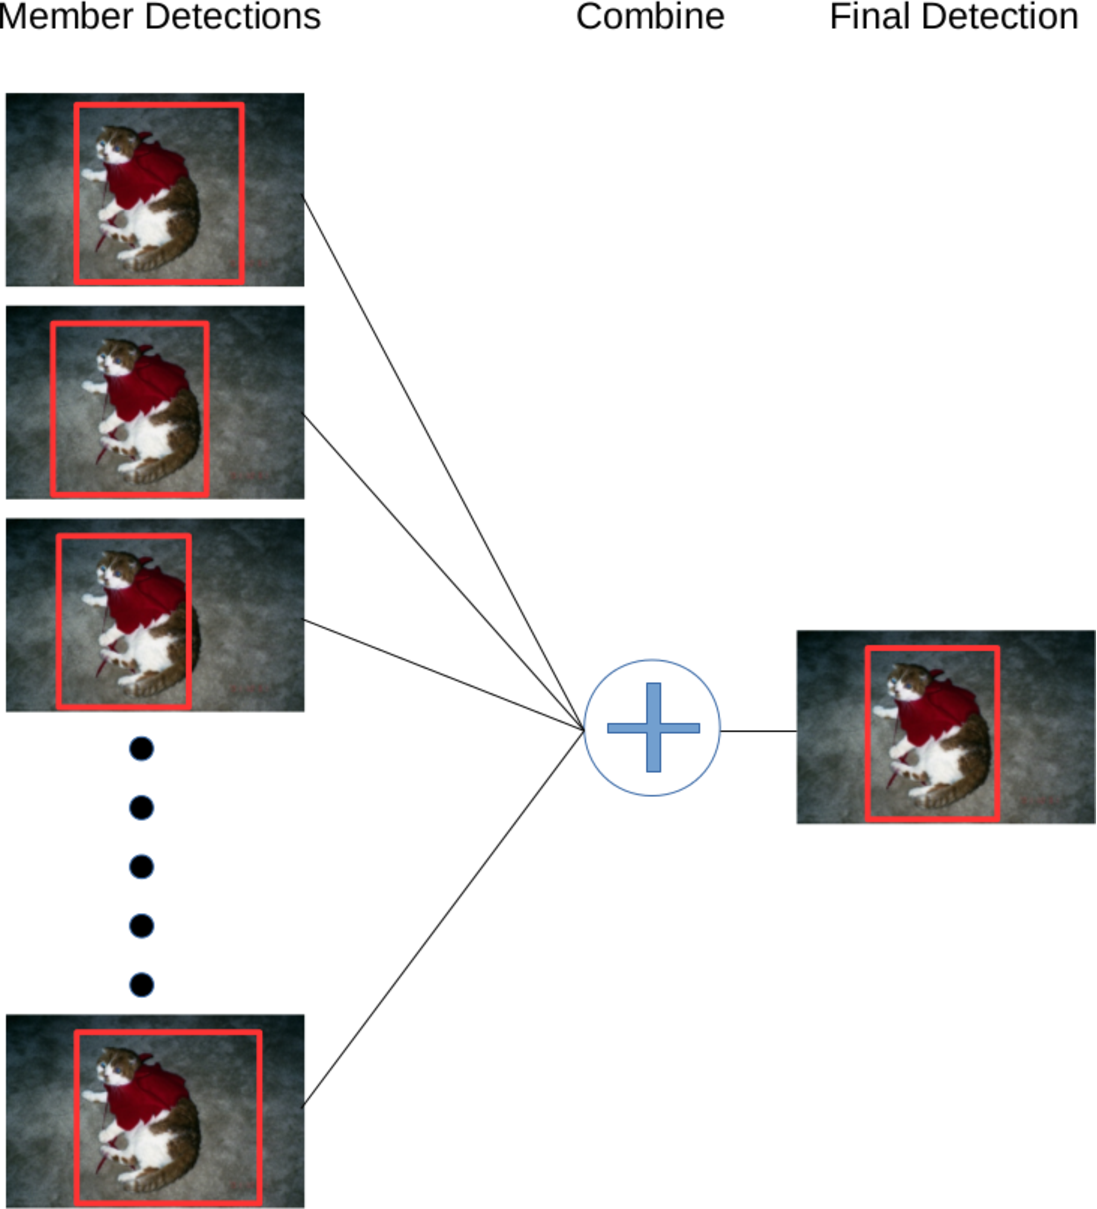
\includegraphics[width=0.5\textwidth]{Figs/ensemble.pdf}
      \caption{General overview for combining detections from different ensemble members. For a given proposal each member produces their respective detections. Then using a combination strategy they are combined for the final detection.}
    \label{fig:ensemble_general}
\end{figure}

A number of different combination strategies will be presented and evaluated in the remainder of this section. 

\subsection{Average Ensemble}
One of the combination strategies is similar to that used when evaluating the expert member results earlier in this chapter. Each of the five ensemble factors are weighted evenly in the overall ensemble. Within each ensemble factor pair, the detection for one of the pairs will be chosen and the other discarded. This is determined by where the given factor lies for the given test image in relation to the training data distribution. For example, if for the given test image it is measured with a deep IQA to have JPEG compression below the threshold used to split the data, then the detection found using the model trained on that data will be used. This results in five detections that will be weighted equally to find the final detection by:

\begin{equation}
  E_{j} = \frac{1}{n} \sum_{i=1}^{n} p_{i,j} 
\end{equation}
where $n$ is the number of detections found by the $n$ ensemble factor, $p$ is the detection result to be averaged and $i$ represents one of the ensemble factors. Finally, $j$ is one of the five values found by each detection, namely the four corners of the bounding-box and the associated confidence.


\subsection{Weighted Average Ensemble}
Each of then 10 trained networks will be used on all object proposals found using the \gls{rpn}. Weights will be distributed evenly across each of the five different types of factors as in the average ensemble. The weighted average ensemble is determined for each bounding-box and the associated confidence by:

\begin{equation}
	E_{j} = \frac{1}{n} \sum_{i=1}^{n} w_ip_{i,j} 
\end{equation}

$w_i$ is the weight for a given detection.Weights are determined in pairs for each of the 5 ensemble factors, where the total sum of weights is equal to $n$. If each detection were to be weighted equally all $w$ would be equal to 1. As the weights are calculated in pairs each ensemble factor is overall weighted equally as the pair of weights can at most be equal to 2. By using this tactic in between the two sets of ensembles for a given factor can be weighted differently but overall each factor is weighted equally.
Weights for a given factor is found according to where the the test image lies for that factors training data distribution. For example, the subsets of training data for Gaussian blur was determined according to the line shown in \figref{blur_dist}. 

\begin{figure}[H]
  \centering
    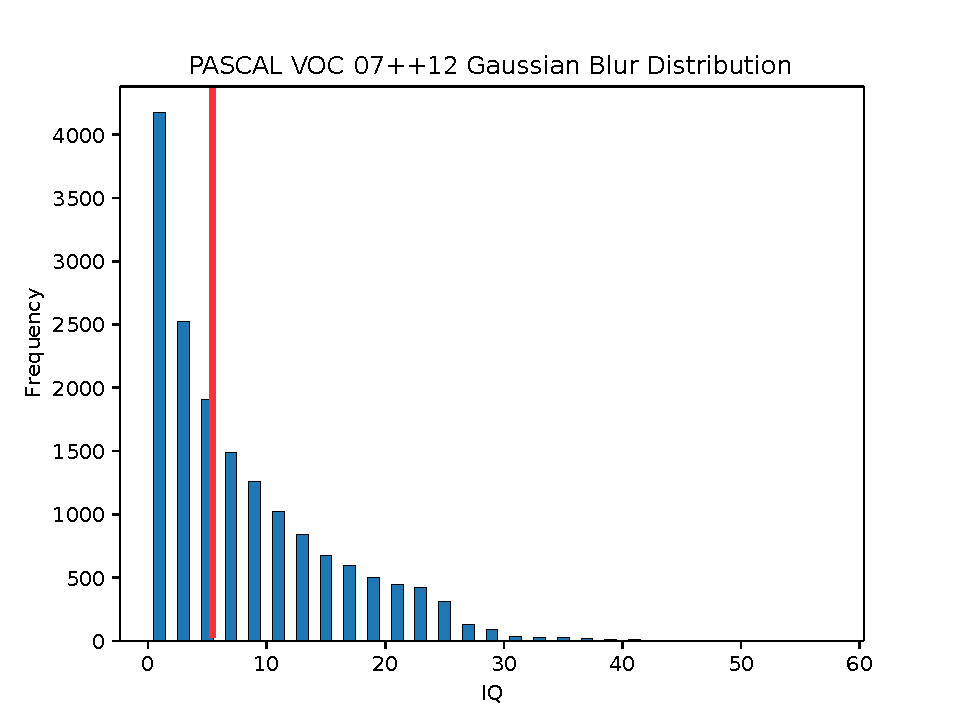
\includegraphics[width=0.8\textwidth]{Figs/GaussianBlurdistred.pdf}
      \caption{Distribution on the 07+12 train set for Gaussian blur found using a trained deep IQA.}
    \label{fig:blur_dist}
\end{figure}

The quality, $q_i$ with respect to blur for a given image is determined using the appropriate deep IQA model, if the quality is below the value used to split the data the weights are calculated for the detection found with the given lower network by:

\begin{equation}
	w_{Lower} = 2 - \frac{median_i - q_i}{median_i - minq_i}
\end{equation}

and the weight for the upper network $w_{Upper}$ by:

\begin{equation}
	w_{Upper} = 2 - w_{Lower}
\end{equation}

where $median_i$ is the value used to split the training data and $minq_i$ is the minimum quality for the given factor in the training set.

However, if the quality is above $split$ the $w_{Upper}$ is calculated by:

\begin{equation}
	w_{Upper} = 2 - \frac{maxq_i - q_i}{maxq_i - median_i}
\end{equation}

and lower weight $w_{Lower}$:

\begin{equation}
	w_{Lower} = 2 - w_{Upper}.
\end{equation}

It should also be noted that outliers are removed for the calculation of $minq_i$ and $maxq_i$ by removing the values below the 1\% and above the 99\% percentile. This ensures that the weighing of factors is not too heavily affected by large or small outlier values.

\section{\uppercase{Experimental Results}}
In this section the results for the two aforementioned ensemble combinations strategies will be presented. Each presentation will be accompanied with the result for the baseline R-FCN ResNet-101 model trained on all of the 07+12 training data and will be dubbed as baseline. The results presented will be on the 2007 \gls{pascalvoc} test set as also shown in earlier preliminary results in this report.
\\\\
The results for both combination strategies can be seen in \tableref{avgres1}.

\begin{table}[h]
\centering
\caption{Results for the two ensemble combination strategies and for the baseline model on the 2007 test set.}
\label{tab:avgres1}
\begin{tabular}{|l|l|}
\hline
\textbf{Method}           & \textbf{AP (\%)} \\ \hline
Average          & 79.21\% \\ \hline
Weighted Average & 79.13\% \\ \hline
Baseline         & \textbf{79.59\%} \\ \hline
\end{tabular}
\end{table}

While neither of the combinations provide an improvement over the baseline method both provide an increase in performance in comparison to the image quality expert results shown in \sectionref{iq_experts}. Here, individual members were 3-4\% worse in performance in comparison to the baseline model on their trained expert areas. Additionally, the weighted average only performs slightly worse than that of the non-weighted version. This is interesting as the intra-factor experts for the image quality factors are similar in performance, however, while disregarding this and weighing models still provides a performance increase.
\\\\
To the evaluate the contribution of both the eight quality factor ensemble members and the two resolution members these were combined separately based on the two strategies. The results for the average ensemble can be seen in \tableref{avgresind} and the weighted ensemble in \tableref{weiavgind}.

\begin{table}[h]
\centering
\caption{Results for the the image quality ensemble members and resolution members individually combined using average strategy on the 2007 test set.}
\label{tab:avgresind}
\begin{tabular}{|l|l|}
\hline
\textbf{Ensemble Members}        & \textbf{AP (\%)} \\ \hline
Image Quality & 78.15\% \\ \hline
Resolution    & 78.13\% \\ \hline
\end{tabular}
\end{table}

\begin{table}[h]
\centering
\caption{Results for the the image quality ensemble members and resolution members individually combined using the weighted average strategy on the 2007 test set.}
\label{tab:weiavgind}
\begin{tabular}{|l|l|}
\hline
\textbf{Ensemble Members}        & \textbf{AP (\%)} \\ \hline
Image Quality & 78.44\% \\ \hline
Resolution    & 75.00\% \\ \hline
\end{tabular}
\end{table}

By separating the quality and resolution members \tableref{avgresind} shows that the performance decreases by over 1\% for both in comparison the the average ensemble result of 79.21\%. This appears to indicate that the two complement each other well and have their own expertises for this problem. \tableref{weiavgind} also shows a decrease in performance when separating the members based on their expertise factors. The weighted average combination strategy does not show as large of a decrease in performance for only image quality as the average combination does, however, there is still a performance drop from 79.13\% to 78.44\%. There is a significant decrease in performance for the two resolution members showing an \gls{ap} of 75.00\% on the test set. This seems to show that the addition of weighing individual detections based on proposal size as a poorer approach. Comparing the two tables seems to indicate that image quality members are well suited to adding a weight to detection. Whereas, the resolution members are better suited to simply taking the detection from the appropriate model. Therefore, combinations of average and weighted average ensembles could be of interest. The results for these can be seen in \tableref{weandavgres}. The two strategies are shown as either Image Quality or Resolution followed by the subscript $_{Avg}$ or $_{WAvg}$ indicating the combination strategies of average or weighted average respectively. 

\begin{table}[h]
\centering
\caption{Results for the the image quality ensemble members and resolution members with both combinations of average and weighted average on the 2007 test set.}
\label{tab:weandavgres}
\begin{tabular}{|l|l|}
\hline
\textbf{Ensemble Members}                  & \textbf{AP (\%)} \\ \hline
Image Quality$_{WAvg}$ / Resolution$_{Avg}$ & \textbf{79.90\%} \\ \hline
Image Quality$_{Avg}$ / Resolution$_{WAvg}$ & 78.71\% \\ \hline
Baseline                          & 79.59\% \\ \hline
\end{tabular}
\end{table}

Results in \tableref{weandavgres} show that by using separate strategies where image quality members are weighted and when resolution members are averaged only increases the performance. Additionally, the performance surpasses the baseline model. The increase is slight from 79.59\% to 79.90\%. However, again it appears that the members of the ensemble compliment each other well both intra-factor and inter-factor. As suspected the opposite strategy of average combination for image quality and weighted average for resolution does not surpass previous results. 
\\\\
The results so far have only been with different combinations of the expert ensemble members. However, another strategy is to include the baseline model trained on all of the 07+12 data. As the baseline model performs well by itself the other ensemble members will act as support, as ideally there are parts of the \gls{pascalvoc} data that they perform better on due to the reduced training variance. The methods for ensemble are used as earlier, except that there is an additional member in the ensemble. Also it should be noted that as there is no complementary member to the baseline. Therefore, its detections are weighted by 1.0 regardless of ensemble combination strategy. Firstly, the results for the average and weighted average ensemble, both with the baseline model can be seen in \tableref{ensemble_base}. The inclusion of the baseline model is shown by the subscript $_{base}$. The table shows that in both strategies the inclusion increases the overall performance. Using the weighted average the performance is increased by 0.22\%. While the average strategy is increased above the baseline result by 0.65\% to 79.86\%.

\begin{table}[h]
\centering
\caption{Results for the two ensemble combination strategies and for the baseline model on the 2007 test set. Shown is both the results with the expert ensemble members only and experts plus the baseline model.}
\label{tab:ensemble_base}
\begin{tabular}{|l|l|}
\hline
\textbf{Method}           & \textbf{AP (\%)} \\ \hline
Average          & 79.21\% \\ \hline
Average$_{base}$          & \textbf{79.86\%} \\ \hline
Weighted Average & 79.13\% \\ \hline
Weighted Average$_{base}$ & 79.35\% \\ \hline
Baseline         & 79.59\% \\ \hline
\end{tabular}
\end{table}

Next the addition of the baseline model with respective to each ensemble factor using the average ensemble strategy can be seen in \tableref{ensembleavg_base}. Both factors have a significant increase in \gls{ap} performance with the extra ensemble member. The image quality experts gain 0.77\%, while the two resolution members have their performance increased by 1.96\%. The result of 80.09 is higher than the result shown in \tableref{weandavgres} even without having members trained towards image quality factors.

\begin{table}[h]
\centering
\caption{Results for the the image quality ensemble members and resolution members individually combined using average strategy on the 2007 test set. Shown is both the results with the expert ensemble members only and experts plus the baseline model.}
\label{tab:ensembleavg_base}
\begin{tabular}{|l|l|}
\hline
\textbf{Ensemble Members}        & \textbf{AP (\%)} \\ \hline
Image Quality & 78.15\% \\ \hline
Image Quality$_{base}$ & 78.92\% \\ \hline
Resolution    & 78.13\% \\ \hline
Resolution$_{base}$    & \textbf{80.09\%} \\ \hline
Baseline         & 79.59\% \\ \hline
\end{tabular}
\end{table}

Adding the baseline model to the factors and using the weighted average strategy does not result in an improvement over the baseline result as shown in \tableref{ensemblewavg_base}. However, both factors see a larger increase in performance than that of the average combination in \tableref{ensembleavg_base}. Image quality performance is increased by 0.71\% and resolution members increase by 3.21\%. Clearly regardless of ensemble strategy the addition of the baseline model aids in overall object detection on \gls{pascalvoc}.

\begin{table}[h]
\centering
\caption{Results for the the image quality ensemble members and resolution members individually combined using weighted average strategy on the 2007 test set.  Shown is both the results with the expert ensemble members only and experts plus the baseline model.}
\label{tab:ensemblewavg_base}
\begin{tabular}{|l|l|}
\hline
\textbf{Ensemble Members}        & \textbf{AP (\%)} \\ \hline
Image Quality & 78.44\% \\ \hline
Image Quality$_{base}$ & 79.15\% \\ \hline
Resolution    & 75.00\% \\ \hline
Resolution$_{base}$    & 78.21\% \\ \hline
Baseline         & \textbf{79.59\%} \\ \hline
\end{tabular}
\end{table}

While improvements are seen for both strategies with the addition of baseline, the tendency is still that the resolution members perform best with the average ensemble and image quality with weighted average. Therefore, the two combinations of ensembles with the addition were tested. This is shown in \tableref{ensemble_comb_base} and shown is that this provided the best result of any ensemble combination. Image quality with the weighted average and resolution with average ensemble results in 80.15\%, an increase of 0.56\% in comparison to the baseline \gls{rfcn}.

\begin{table}[h]
\centering
\caption{Results for the the image quality ensemble members and resolution members with both combinations of average and weighted average on the 2007 test set.  Shown is both the results with the expert ensemble members only and experts plus the baseline model.}
\label{tab:ensemble_comb_base}
\begin{tabular}{|l|l|}
\hline
\textbf{Ensemble Members}                  & \textbf{AP (\%)} \\ \hline
Image Quality$_{WAvg}$ / Resolution$_{Avg}$  & 79.90\% \\ \hline
Image Quality$_{WAvg}$ / Resolution$_{Avg}$ $_{base}$ & \textbf{80.15\%} \\ \hline
Image Quality$_{Avg}$ / Resolution$_{WAvg}$ & 78.71\% \\ \hline
Image Quality$_{Avg}$ / Resolution$_{WAvg}$ $_{base}$ & 79.10\% \\ \hline
Baseline                          & 79.59\% \\ \hline
\end{tabular}
\end{table}


The \gls{ap} results for each categories for best performing ensembles are shown in \tableref{resbaseclasses} and \tableref{bestbaseclasses}. The tables show results for the baseline model, the given ensemble method and the difference between the two for a given class. For the Resolution$_{base}$ ensemble, which had an overall increase of 0.5\%, 13 of the 20 classes had an improvement compared to the baseline model. As seen in \tableref{resbaseclasses} the largest increases were for the TV class with 2.77\%, train 2.53\% and sofa 1.64\%. The classes with the largest decrease in performance were horse falling by 2.21\% and cow with 1.04\%


\begin{table}[h]
\centering
\caption{Results for the individual classes in the 2007 test set. Shown are the results for the baseline model and Resolution$_{base}$. Additionally the difference between the two methods are presented for a given class.}
\label{tab:resbaseclasses}
\resizebox{\columnwidth}{!}{%
\begin{tabular}{lllllllllll}
\hline
\multicolumn{1}{|l|}{\textbf{Model}}                                                                           & \multicolumn{1}{l|}{\textbf{aero}}  & \multicolumn{1}{l|}{\textbf{bike}}  & \multicolumn{1}{l|}{\textbf{bird}}  & \multicolumn{1}{l|}{\textbf{boat}}  & \multicolumn{1}{l|}{\textbf{bottle}} & \multicolumn{1}{l|}{\textbf{bus}}   & \multicolumn{1}{l|}{\textbf{car}}   & \multicolumn{1}{l|}{\textbf{cat}}   & \multicolumn{1}{l|}{\textbf{chair}} & \multicolumn{1}{l|}{\textbf{cow}}   \\ \hline
\multicolumn{1}{|l|}{Baseline}        & \multicolumn{1}{l|}{80.53} & \multicolumn{1}{l|}{\textbf{84.59}} & \multicolumn{1}{l|}{79.89} & \multicolumn{1}{l|}{71.52} & \multicolumn{1}{l|}{67.54}  & \multicolumn{1}{l|}{87.22} & \multicolumn{1}{l|}{\textbf{87.59}} & \multicolumn{1}{l|}{87.98} & \multicolumn{1}{l|}{65.15} & \multicolumn{1}{l|}{\textbf{87.11}} \\ \hline
\multicolumn{1}{|l|}{Resolution$_{base}$} & \multicolumn{1}{l|}{\textbf{82.04}} & \multicolumn{1}{l|}{84.21} & \multicolumn{1}{l|}{\textbf{80.14}} & \multicolumn{1}{l|}{\textbf{72.08}} & \multicolumn{1}{l|}{\textbf{69.05}}  & \multicolumn{1}{l|}{\textbf{87.86}} & \multicolumn{1}{l|}{87.56} & \multicolumn{1}{l|}{\textbf{89.28}} & \multicolumn{1}{l|}{\textbf{66.01}} & \multicolumn{1}{l|}{86.07} \\ \hline
\multicolumn{1}{|l|}{Difference}     & \multicolumn{1}{l|}{+1.51} & \multicolumn{1}{l|}{-0.58} & \multicolumn{1}{l|}{+0.25} & \multicolumn{1}{l|}{+0.56} & \multicolumn{1}{l|}{+1.51}  & \multicolumn{1}{l|}{+0.64} & \multicolumn{1}{l|}{-0.03} & \multicolumn{1}{l|}{+1.30} & \multicolumn{1}{l|}{+0.86} & \multicolumn{1}{l|}{-1.04} \\ \hline
                                      &                            &                            &                            &                            &                             &                            &                            &                            &                            &                            \\ \hline
\multicolumn{1}{|l|}{\textbf{Model}}                                                                           & \multicolumn{1}{l|}{\textbf{table}} & \multicolumn{1}{l|}{\textbf{dog}}   & \multicolumn{1}{l|}{\textbf{horse}} & \multicolumn{1}{l|}{\textbf{mbike}} & \multicolumn{1}{l|}{\textbf{person}} & \multicolumn{1}{l|}{\textbf{plant}} & \multicolumn{1}{l|}{\textbf{sheep}} & \multicolumn{1}{l|}{\textbf{sofa}}  & \multicolumn{1}{l|}{\textbf{train}} & \multicolumn{1}{l|}{\textbf{tv}}    \\ \hline
\multicolumn{1}{|l|}{Baseline}        & \multicolumn{1}{l|}{\textbf{73.66}} & \multicolumn{1}{l|}{88.61} & \multicolumn{1}{l|}{\textbf{87.83}} & \multicolumn{1}{l|}{83.21} & \multicolumn{1}{l|}{79.87}  & \multicolumn{1}{l|}{\textbf{54.60}} & \multicolumn{1}{l|}{\textbf{84.07}} & \multicolumn{1}{l|}{80.03} & \multicolumn{1}{l|}{83.60} & \multicolumn{1}{l|}{77.17} \\ \hline
\multicolumn{1}{|l|}{Resolution$_{base}$} & \multicolumn{1}{l|}{73.04} & \multicolumn{1}{l|}{\textbf{89.10}} & \multicolumn{1}{l|}{85.62} & \multicolumn{1}{l|}{\textbf{83.59}} & \multicolumn{1}{l|}{\textbf{79.95}}  & \multicolumn{1}{l|}{54.30} & \multicolumn{1}{l|}{83.63} & \multicolumn{1}{l|}{\textbf{81.67}} & \multicolumn{1}{l|}{\textbf{86.13}} & \multicolumn{1}{l|}{\textbf{80.47}} \\ \hline
\multicolumn{1}{|l|}{Difference}     & \multicolumn{1}{l|}{-0.62} & \multicolumn{1}{l|}{+0.49} & \multicolumn{1}{l|}{-2.21} & \multicolumn{1}{l|}{+0.38} & \multicolumn{1}{l|}{+0.08}  & \multicolumn{1}{l|}{-0.30} & \multicolumn{1}{l|}{-0.44} & \multicolumn{1}{l|}{+1.64} & \multicolumn{1}{l|}{+2.53} & \multicolumn{1}{l|}{+2.77} \\ \hline
\end{tabular}
%
}
\end{table}
 
\tableref{bestbaseclasses} shows that for the Image Quality$_{WAvg}$ / Resolution$_{Avgbase}$ ensemble again 13 of the classes increased in performance. The largest increase were again train and TV with 2.77\% and 2.48\% respectively. Interestingly, the third largest winner with Resolution$_{base}$, sofa, decreased in performance in this instance. Giving an indication that object detection does not improve for all classes with the addition of image quality ensemble members. The worse performers in this instance were table and horse, decreasing by 1.63\% and 0.87\% respectively.


\begin{table}[h]
\centering
\caption{Results for the individual classes in the 2007 test set. Shown are the results for the baseline model and Image Quality$_{WAvg}$ / Resolution$_{Avgbase}$ . Additionally the difference between the two methods are presented for a given class}
\label{tab:bestbaseclasses}
\resizebox{\columnwidth}{!}{%
\begin{tabular}{lllllllllll}
\hline
\multicolumn{1}{|l|}{\textbf{Model}}                                                                           & \multicolumn{1}{l|}{\textbf{aero}}  & \multicolumn{1}{l|}{\textbf{bike}}  & \multicolumn{1}{l|}{\textbf{bird}}  & \multicolumn{1}{l|}{\textbf{boat}}  & \multicolumn{1}{l|}{\textbf{bottle}} & \multicolumn{1}{l|}{\textbf{bus}}   & \multicolumn{1}{l|}{\textbf{car}}   & \multicolumn{1}{l|}{\textbf{cat}}   & \multicolumn{1}{l|}{\textbf{chair}} & \multicolumn{1}{l|}{\textbf{cow}}   \\ \hline
\multicolumn{1}{|l|}{Baseline}                                                                        & \multicolumn{1}{l|}{80.53} & \multicolumn{1}{l|}{84.59} & \multicolumn{1}{l|}{79.89} & \multicolumn{1}{l|}{71.52} & \multicolumn{1}{l|}{67.54}  & \multicolumn{1}{l|}{87.22} & \multicolumn{1}{l|}{\textbf{87.59}} & \multicolumn{1}{l|}{87.98} & \multicolumn{1}{l|}{65.15} & \multicolumn{1}{l|}{\textbf{87.11}} \\ \hline
\multicolumn{1}{|l|}{\begin{tabular}[c]{@{}l@{}}Image Quality$_{WAvg}$ /\\ Resolution$_{Avgbase}$\end{tabular}} & \multicolumn{1}{l|}{\textbf{81.41}} & \multicolumn{1}{l|}{\textbf{85.79}} & \multicolumn{1}{l|}{\textbf{81.09}} & \multicolumn{1}{l|}{\textbf{72.87}} & \multicolumn{1}{l|}{\textbf{69.09}}  & \multicolumn{1}{l|}{\textbf{88.00}} & \multicolumn{1}{l|}{87.42} & \multicolumn{1}{l|}{\textbf{89.12}} & \multicolumn{1}{l|}{\textbf{66.71}} & \multicolumn{1}{l|}{86.72} \\ \hline
\multicolumn{1}{|l|}{Difference}                                                                     & \multicolumn{1}{l|}{+0.88} & \multicolumn{1}{l|}{+1.20} & \multicolumn{1}{l|}{+1.20} & \multicolumn{1}{l|}{+1.35} & \multicolumn{1}{l|}{+1.55}  & \multicolumn{1}{l|}{+0.78} & \multicolumn{1}{l|}{-0.17} & \multicolumn{1}{l|}{+1.14} & \multicolumn{1}{l|}{+1.56} & \multicolumn{1}{l|}{-0.39} \\ \hline
                                                                                                      &                            &                            &                            &                            &                             &                            &                            &                            &                            &                            \\ \hline
\multicolumn{1}{|l|}{\textbf{Model}}                                                                           & \multicolumn{1}{l|}{\textbf{table}} & \multicolumn{1}{l|}{\textbf{dog}}   & \multicolumn{1}{l|}{\textbf{horse}} & \multicolumn{1}{l|}{\textbf{mbike}} & \multicolumn{1}{l|}{\textbf{person}} & \multicolumn{1}{l|}{\textbf{plant}} & \multicolumn{1}{l|}{\textbf{sheep}} & \multicolumn{1}{l|}{\textbf{sofa}}  & \multicolumn{1}{l|}{\textbf{train}} & \multicolumn{1}{l|}{\textbf{tv}}    \\ \hline
\multicolumn{1}{|l|}{Baseline}                                                                        & \multicolumn{1}{l|}{\textbf{73.66}} & \multicolumn{1}{l|}{88.61} & \multicolumn{1}{l|}{\textbf{87.83}} & \multicolumn{1}{l|}{83.21} & \multicolumn{1}{l|}{79.87}  & \multicolumn{1}{l|}{\textbf{54.60}} & \multicolumn{1}{l|}{\textbf{84.07}} & \multicolumn{1}{l|}{\textbf{80.03}} & \multicolumn{1}{l|}{83.60} & \multicolumn{1}{l|}{77.17} \\ \hline
\multicolumn{1}{|l|}{\begin{tabular}[c]{@{}l@{}}Image Quality$_{WAvg}$ /\\ Resolution$_{Avgbase}$\end{tabular}} & \multicolumn{1}{l|}{72.03} & \multicolumn{1}{l|}{\textbf{88.69}} & \multicolumn{1}{l|}{86.96} & \multicolumn{1}{l|}{\textbf{84.24}} & \multicolumn{1}{l|}{\textbf{80.09}}  & \multicolumn{1}{l|}{53.74} & \multicolumn{1}{l|}{83.28} & \multicolumn{1}{l|}{79.88} & \multicolumn{1}{l|}{\textbf{86.28}} & \multicolumn{1}{l|}{\textbf{79.65}} \\ \hline
\multicolumn{1}{|l|}{Difference}                                                                     & \multicolumn{1}{l|}{-1.63} & \multicolumn{1}{l|}{+0.08} & \multicolumn{1}{l|}{-0.87} & \multicolumn{1}{l|}{+1.03}  & \multicolumn{1}{l|}{+0.22}  & \multicolumn{1}{l|}{-0.86} & \multicolumn{1}{l|}{-0.79} & \multicolumn{1}{l|}{-0.15} & \multicolumn{1}{l|}{+2.68} & \multicolumn{1}{l|}{+2.48} \\ \hline
\end{tabular}
%
}
\end{table}


Finally, two examples of detections can be seen in \figref{boatres} and \figref{trainres}. For both figures, on the left is the full size image and right a zoomed version of the object and detections. The detections shown are for the ground truth annotation, baseline, Resolution$_{base}$ (Res) and Image Quality$_{WAvg}$ / Resolution$_{Avgbase}$ (IQ / Res). Additionally, shown in parentheses in the legend is the \gls{iou} between the ground truth and detection for the given method. Additional examples of detections can be seen in \sectionref{detectionappendix}.
For the boat detection in \figref{boatres}, both ensemble methods increase the \gls{iou} significantly compared to the baseline detection. The \gls{iou} with the Resolution$_{base}$ is 0.045 higher at 0.845. The Image Quality$_{WAvg}$ / Resolution$_{Avgbase}$ detection matches even better with 0.061 higher intersection. The difference in the results seems to be largely due to the closer bounding box towards the right side of the boat, with the Image Quality$_{WAvg}$ / Resolution$_{Avgbase}$ fitting especially well.


\begin{figure*}[!h]
\minipage{0.5\textwidth}
  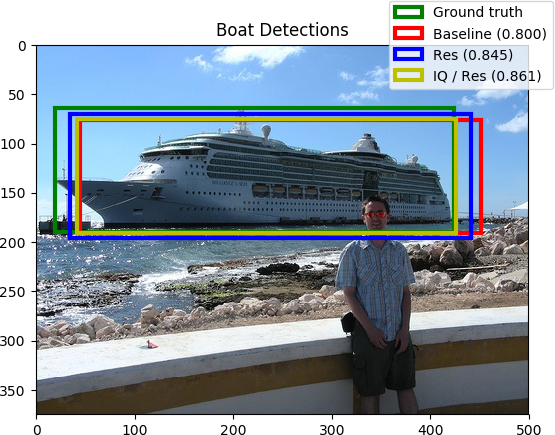
\includegraphics[width=\linewidth]{Figs/000069res.png}
  \caption*{}\label{fig:}
\endminipage\hfill
\minipage{0.5\textwidth}
  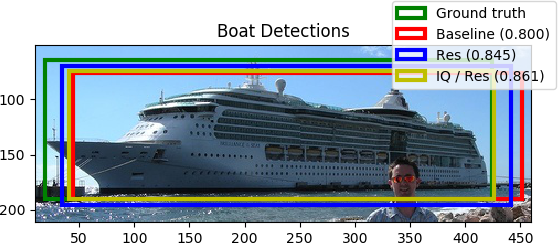
\includegraphics[width=\linewidth]{Figs/000069reszoom.png}
  \caption*{}\label{fig:}
\endminipage\hfill
\caption{Detections for the boat class from an image in the 2007 test set. Shown are the bounding boxes for the ground truth annotation, baseline, Resolution$_{base}$ (Res) and Image Quality$_{WAvg}$ / Resolution$_{Avgbase}$ (IQ / Res). The \gls{iou} between the ground truth and bounding box is shown in parentheses for each method.}
\label{fig:boatres}
\end{figure*}

\figref{trainres} is an example of a relatively small object in an image. In this instance the best fitting detection is from the Resolution$_{base}$ ensemble with an \gls{iou} of 0.825. An increase of 0.071 compared to the detection with the baseline model. The Image Quality$_{WAvg}$ / Resolution$_{Avgbase}$ also has a better fitting detection with an \gls{iou} of 0.803. The improvement for both ensembles seem to be towards to top of the train  where both bounding boxes fit the ground truth better than the baseline detection.
Again, both models had significant improvements for the train class compared to the baseline model.

 
 \begin{figure*}[!h]
\minipage{0.5\textwidth}
  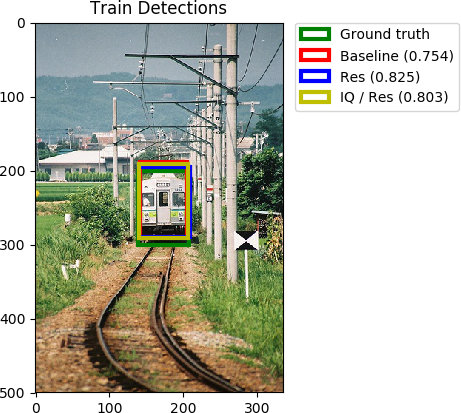
\includegraphics[width=\linewidth]{Figs/000002_res.png}
  \caption*{}\label{fig:}
\endminipage\hfill
\minipage{0.5\textwidth}
  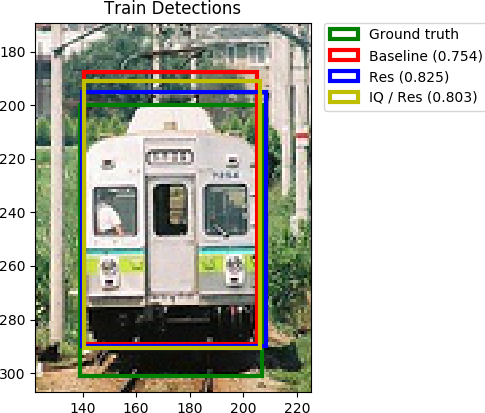
\includegraphics[width=\linewidth]{Figs/000002_reszoom.png}
  \caption*{}\label{fig:}
\endminipage\hfill
\caption{Detections for the boat class from an image in the 2007 test set. Shown are the bounding boxes for the ground truth annotation, baseline, Resolution$_{base}$ (Res) and Image Quality$_{WAvg}$ / Resolution$_{Avgbase}$ (IQ / Res). The \gls{iou} between the ground truth and bounding box is shown in parentheses for each method.}
\label{fig:boatres}
\end{figure*}





\section{\uppercase{Discussion}}

\section{\uppercase{Conclusion}}

\section*{\uppercase{Acknowledgements}}

\noindent If any, should be placed before the references section
without numbering. To do so please use the following command:
\textit{$\backslash$section*\{ACKNOWLEDGEMENTS\}}


\vfill
\bibliographystyle{apalike}
{\small
\bibliography{example}}


\section*{\uppercase{Appendix}}

\noindent If any, the appendix should appear directly after the
references without numbering, and not on a new page. To do so please use the following command:
\textit{$\backslash$section*\{APPENDIX\}}

\vfill

\end{document}

